\documentclass[12pt]{article}
\RequirePackage{amsthm,amsmath,amsbsy,amsfonts}
\usepackage{graphicx}
%\usepackage{enumerate}
\usepackage{natbib}
\usepackage{url} % not crucial - just used below for the URL 
\usepackage{placeins}
\usepackage{algorithm}
\usepackage{algpseudocode}
%\pdfminorversion=4
% NOTE: To produce blinded version, replace "0" with "1" below.
\newcommand{\blind}{0}

% DON'T change margins - should be 1 inch all around.
\addtolength{\oddsidemargin}{-.5in}%
\addtolength{\evensidemargin}{-.5in}%
\addtolength{\textwidth}{1in}%
\addtolength{\textheight}{1.3in}%
\addtolength{\topmargin}{-.8in}%


\begin{document}
	
	%\bibliographystyle{natbib}
	
	\def\spacingset#1{\renewcommand{\baselinestretch}%
		{#1}\small\normalsize} \spacingset{1}
	
	
	%%%%%%%%%%%%%%%%%%%%%%%%%%%%%%%%%%%%%%%%%%%%%%%%%%%%%%%%%%%%%%%%%%%%%%%%%%%%%%
	
	\if0\blind
	{
		\title{\bf Drift Removal for Time Series Data Using Quantile Trend Filtering}
		\author{Halley Brantley\thanks{
				Department of Statistics, North Carolina State University, Raleigh, NC 27695 (E-mail: hlbrantl@ncsu.edu)} \,
			Joseph Guinness\thanks{
				Department of Biological Statistics and Computational Biology, Cornell University, Ithaca, NY 14853 (E-mail: guinness@cornell.edu )} \,
			and
			%    and
			Eric C. Chi\thanks{Department of Statistics, North Carolina State University, Raleigh, NC 27695 (E-mail: eric$\_$chi@ncsu.edu).}    \\}
		\date{}
		\maketitle
	} \fi
		
	\if1\blind
	{
		\bigskip
		\bigskip
		\bigskip
		\begin{center}
			{\LARGE\bf Title}
		\end{center}
		\medskip
	} \fi
	
	\bigskip
	\begin{abstract}
		The text of your abstract.  200 or fewer words.
	\end{abstract}
	
	\noindent%
	{\it Keywords:}  3 to 6 keywords, that do not appear in the title
	\vfill
	
	\newpage
	\spacingset{1.5} % DON'T change the spacing!
	\section{Introduction}
	\label{sec:intro}
	
	In many applications spanning the fields of chemistry \citep{Ning2014}, macroeconomics \citep{yamada2017estimating}, environmental science \citep{brantley2014mobile}, and medical sciences \citep{pettersson2013algorithm, marandi2015qualitative}, scalar time series are observed and assumed to consist of a slowly varying trend other more rapidly varying components. Given observations $y(t)$, with $t=1, ..., N$, \cite{Kim2009} proposed using \textit{$\ell_1$ trend filtering} to estimate trends that are smooth in the sense of being piecewise linear or piecewise polynomial. \cite{Tib2014} then discovered that empirically the trend filtering estimates adapt to the local level of smoothness much better than the more common smoothing splines. In the trend filtering problem \citep{Kim2009, Tib2014}, the trend, $\theta \in \mathbb{R}^n$, is estimated by solving the following convex problem.
	\begin{eqnarray}
	\underset{\theta}{\arg\min}\; \frac{1}{2} \lVert y - \theta \rVert_2^2 + \lambda \lVert \mathbf{D}^{(k+1)}\theta \rVert_1,
	\end{eqnarray}
	where $\lambda \geq 0$ is a regularization parameter and the matrix $\mathbf{D}^{(k+1)} \in \mathbb{R}^{(n - k -1) \times n}$ is the discrete difference operator of order $k+1$. To understand the purpose of penalizing $\mathbf{D}^{(k+1)}$ consider the difference operator when $k = 0$.
	\begin{eqnarray}
	\mathbf{D}^{(1)} = \begin{pmatrix}
	-1 & 1 & 0 & \cdots & 0 & 0 \\
	0 & -1 & 1 & \cdots & 0 & 0 \\
	\vdots & & & & & \\
	0 & 0 & 0 & \cdots & -1 & 1 \\
	\end{pmatrix}
	\end{eqnarray}
	Thus, $\lVert \mathbf{D}^{(1)}\theta \rVert_1 = \sum_{i=1}^{n-1} \lvert \theta_i - \theta_{i+1} \rvert$ which is just total variation denoising in one dimension. The penalty incentivizes solutions which are piece-wise constant. For $k \geq 1$, the difference operator $\mathbf{D}^{(k+1)} \in \mathbb{R}^{(n-k-1) \times n}$ is defined recursively as follows
	\begin{eqnarray}
	\mathbf{D}^{(k+1)} & = & \mathbf{D}^{(1)}\mathbf{D}^{(k)}.
	\end{eqnarray}
	By penalizing the $k+1$ fold composition of the discrete difference operator, we obtain solutions which are piecewise polynomials of order $k$. Trend filtering provides excellent estimates of trends when the only components of the time series are the trend and random noise (Fig. \ref{fig:trendfilter}). In some cases, time series may also include a rapidly varying signal component in addition to the trend and noise, in these cases the trend filtering estimate over-estimate the trend in the places where signal is present (Fig. \ref{fig:trendfilter}).  
	   	
	\begin{figure}
		\centering
		\caption{Examples of trend filtering solutions. The true trend is shown in black, while the .estimated trend is shown in red.}
		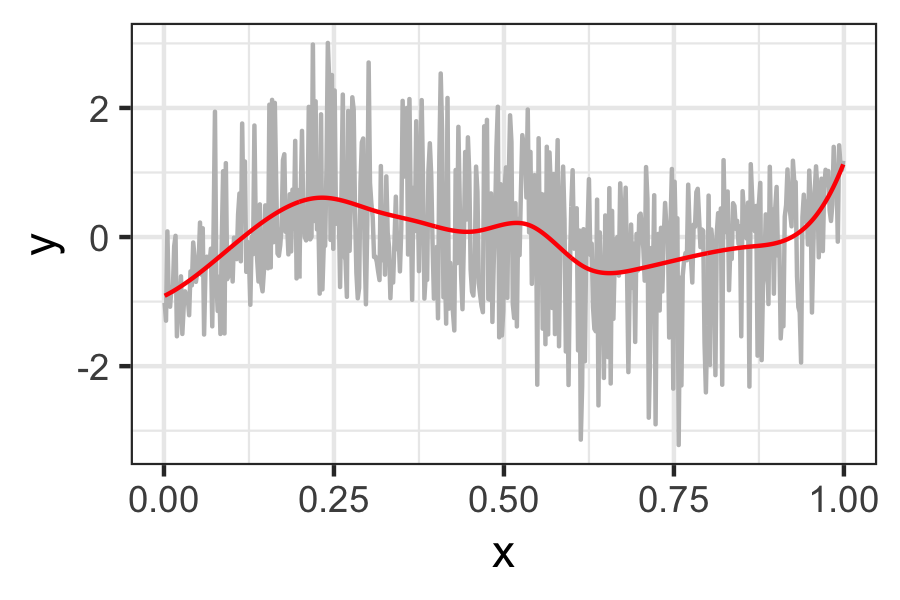
\includegraphics[width = 0.45\linewidth]{Figures/trend_filter_eg1.png}
		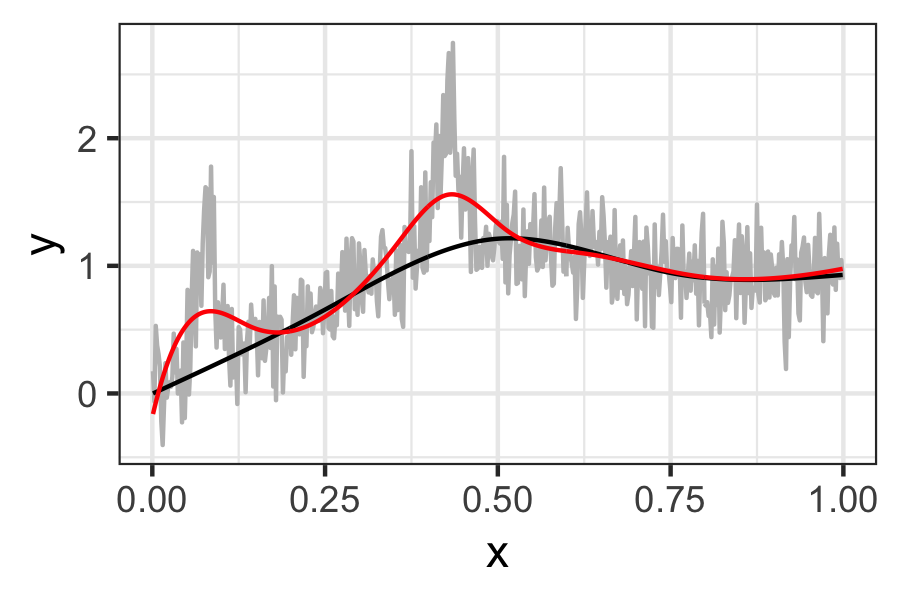
\includegraphics[width = 0.45\linewidth]{Figures/trend_filter_eg2.png}
		\label{fig:trendfilter}
	\end{figure}
	 
	
	One application in which the observed time series consists of a slowly varying trend, non-negative signal, and rapidly varying noise is the output of low cost air quality sensors. The use of low-cost, portable, air quality sensors has increased dramatically in the last decade. These sensors can provide an un-calibrated measure of a variety of pollutants in near real time, but deriving meaningful information from sensor data remains a challenge \citep{snyder2013changing}. The ``SPod" is a low-cost sensor currently being investigated by researchers at the U.S. Environmental Protection Agency to detect volatile organic compound (VOC) emissions from industrial facilities \citep{thoma2016south}. To reduce cost and power consumption of the SPod, the relative humidity of the air presented to the photoionization detectors (PIDs) is not controlled and as a result the output signal exhibits a slowly varying baseline drift on the order of minutes to hours (Fig. \ref{fig:raw_spod}). 
	 
	\begin{figure}[b!]
		\caption{Example of 3 co-located SPod PID sensor readings.}
		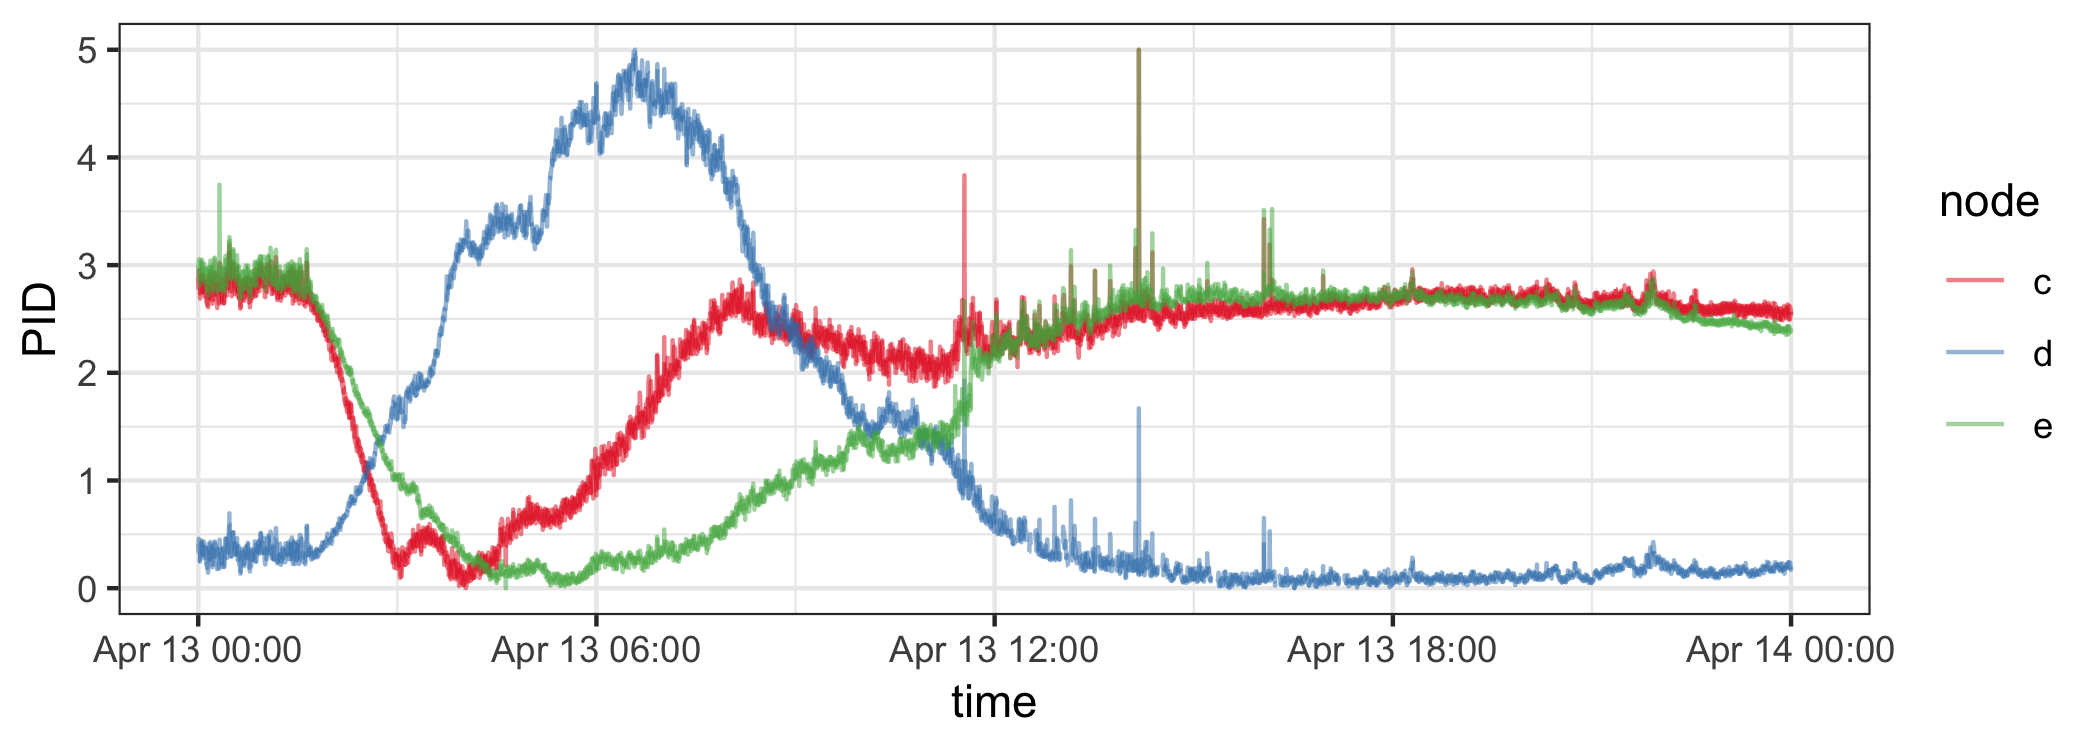
\includegraphics[width = \linewidth]{Figures/uncorrected_data.png}
		\label{fig:raw_spod}
	\end{figure}
   	
	
	In this application, as well as those described in \cite{Ning2014}, \cite{marandi2015qualitative}, and \cite{pettersson2013algorithm}, it is not the mean trend that is desired but rather the baseline trend, which we can think of as the trend in a low quantile of the data.  \cite{Koenker1978} were the first to propose substituting the squared loss used in regression with the check loss function  (Eq. \ref{eq1}) to estimate a conditional quantile instead of the conditional mean. 
	
	\begin{equation}
	\label{eq1}
	 \rho_{\tau}(z) = \sum_{i=1}^n z_i(1-\mathbf{I}(z_i<0)).
	\end{equation}
	
	A variety of approaches have been proposed for estimating quantile trends.  The regression vector $\theta$ is estimated by finding the minimizer of $\rho_{\tau}(y-X\theta)$ where is the check-loss function and $\mathbf{I}$ is the indicator function.   \cite{nychka1995nonparametric} estimated quantile splines by combining the smoothing spline penalty commonly used in non-parametric regression with the check-loss function used in qunatile regression:
	
	\begin{equation*}
	\rho_{\tau}(Y - f) + \lambda\int (f''(t))^2 dt, 
 	\end{equation*}
	
	where $Y(t)$ is a response variable observed at time $t$, $f(t)$ is a smooth function of time and $\lambda$ is a tuning parameter that controls the degrees of smoothing. 


	We propose to use the trend filtering penalty with the check loss function to produce a non-parametric quantile regression estimate for removing trends in time series. The formulation was proposed by \cite{Kim2009} as a possible extension of $\ell_1$-trend filtering but not studied. Moreover we extend the basic framework to ensure non-crossing while modeling multiple quantiles. We also implement a parallel ADMM algorithm for series that are too large to be computed simultaneously and proposed a modified criteria for choosing the smoothing parameter. We demonstrate through simulation studies that our proposed model provides better or comparable estimates of non-parametric quantile trends than existing methods and is a more effective method of drift removal for low-cost air quality sensors. 
	

	\section{Methods}
	
	\subsection{Quantile Trend Filtering}
	
	We combine the ideas of quantile regression and trend filtering, namely consider the case where the design $\mathbf{X}$ is the identity matrix. For a single quantile level $\tau$ the estimation of the quantile trend filtering model can be posed as the following optimization problem.
	\begin{eqnarray}
	\label{eq:quantile_trend}
	\underset{\theta}{\min}\; \rho_\tau(y - \theta) + \lambda \lVert \mathbf{D}^{(k+1)} \theta \rVert_1,
	\end{eqnarray}
	where $\lambda$ is a non-negative regularization parameter. We address the problem of choosing $\lambda$ in Section \ref{sec:lambda_choice}. As with the classic quantile regression, the quantile trend filtering problem is a linear program which can be solved by a number of free or commercial solvers. In many cases, including ours, we are interested in estimating multiple quantiles simultaneously. We also want to ensure that our quantile estimates are valid by enforcing the constraint that if $\tau_2 > \tau_1$ then $Q(\tau_2) \ge Q(\tau_1)$. Given quantiles $\{\tau_1, ..., \tau_J\}$ such that $\tau_1 < \tau_2 < ... < \tau_J$, the optimization problem becomes 
	
	\begin{eqnarray}
	\label{eq:noncross_trend}
	\underset{\theta_1, ..., \theta_J}{\min}\; \sum_{j=1}^J \left [\rho_{\tau_j}(y - \theta_{j}) + 
	\lambda_j \lVert \mathbf{D}^{(k+1)} \theta_j \rVert_1 \right ] \\
	 \text{subject to: }\; \theta_{1i} \le \theta_{2i} \le ... \le \theta_{Ji} \text{ for all } i,
	\end{eqnarray}
	
	where $\theta_j \in \mathcal{R}^n$. The additional constraints are linear in the parameters so the non-crossing quantile trends can still be estimated by a number of available solvers. In the rest of this paper we rely on the commercial solver Gurobi \citep{gurobi}. 
	
	The number of parameters to be estimated is equal to the number of observations multiplied by the number of quantiles of interest. As the size of the data and the number of quantiles grows, all solvers will eventually break. 
	
	\subsection{ADMM for Big Data}
	
	To our knowledge, no one has addressed the problem of finding smooth quantile trends of series that are too large to be processed simultaneously. We propose an alternating direction method of multipliers (ADMM) algorithm for solving large problems in a piecewise fashion. The ADMM algorithm is fully described by \cite{boyd2011distributed, gabay1975dual, glowinski1975approximation}. We apply the consensus ADMM algorithm to the the quantile regression trend filtering problem given in Eq. \ref{eq:quantile_trend}, by dividing our observed series $y(t)$ with $t = \{1, ..., N\}$ into overlapping windows 
	
	\begin{align*}
	\begin{cases}
	y_1(t) = y(t) & \mbox{if~~} 1 \le t \le u_{1}\\
	y_2(t) = y(t) & \mbox{if~~} l_{2} \le t \le u_{2} \\
	y_3(t) = y(t) & \mbox{if~~} l_{3} \le t \le u_{3} \\
	\cdots & \\
	y_M(t) = y(t) & \mbox{if~~} l_{M} \le t \le  N\\
	\end{cases}
	\end{align*}

	 with boundaries $1 < l_{2} < u_{1} < l_{3} < u_{2} < l_{4} < u_{3} < ...< N$. Given quantiles $\tau_1 < ... < \tau_J$ to be estimated we define $\theta_{j,m}(t)$ as the value of the $\tau_j$\textsuperscript{th} quantile trend in window $M$ at time point $t$. In order to write out the constraint the that overlapping sections must be equal we define a consensus variable
	 
	 \begin{align}
		 \bar{\theta}_{j,m} =&  g(\theta_{j, m-1}, \theta_{j,m}, \theta_{j,m+1}) \\
		 =& \begin{cases} 
			 \frac{\theta_{j,m-1}(t)+\theta_{j,m}(t)}{2} & \mbox{if~~} l_{m} \le t \le u_{m-1}  \\
			 \theta_{j,m}(t) & \mbox{if~~} u_{m-1} \le t \le l_{m+1}  \\
			 \frac{\theta_{j,m}(t)+\theta_{j,m+1}(t)}{2} & \mbox{if~~} l_{m+1} \le t \le u_{m}  
			 \end{cases},
	\end{align}
	defining $\theta_{j,M+1} = \theta_{j,M}$ and $\theta_{j,0} = \theta_{j,1}$. Our windowed quantile trend optimization problem can then be written as 
	 \begin{align}
		 \label{eq:quantile_windows}
		 &\sum_{m=1}^M\underset{\theta_{1,m}, ..., \theta_{J,m}}{\min}\; \sum_{j=1}^J \left [\rho_{\tau_j}(y_m - \theta_{j,m}) + 
		 \lambda_j \lVert \mathbf{D}^{(k+1)} \theta_{j,m} \rVert_1 \right ] \\
		 &\text{subject to: }\; \theta_{1,m}(t) \le \theta_{2,m}(t) \le ... \le \theta_{J,m}(t) \text{ for all } m,t \\
		 &\text{subject to: }\; \theta_{j,m}(t) = \bar{\theta}_{j,m}(t) \text{ for all } j, m, t
	 \end{align}
	 Given values for the Lagrange multiplier $\omega_{j,m}$ and the consensus variable $\bar{\theta}_{j,m}$ we can write the augmented Lagrangian for finding the trends in window $m$:
	 \begin{equation}
	 \mathcal{L}(\theta_{j,m}, \bar{\theta}_{j,m}, \omega_{j,m}) = \sum_{j=1}^J\rho_{\tau_j}(y_m - \theta_{j,m})+\lambda \lVert \mathbf{D}^{(k+1)}\theta_{j,m}\rVert_1 +  \omega_{j,m}^T(\theta_{j,m} - \bar{\theta}_{j,m}) + 
	 \frac{\gamma}{2}||\theta_{j,m} - \bar{\theta}_{j,m}||_2^2
	 \end{equation}
	 
	 We then estimate the trend separately in each window while constraining the overlapping pieces of the trends to be equal according the algorithm 1. 
	 
	\begin{figure}[!h] 
		\centering
		\caption{Window boundaries and trends fit separately in each window.}
		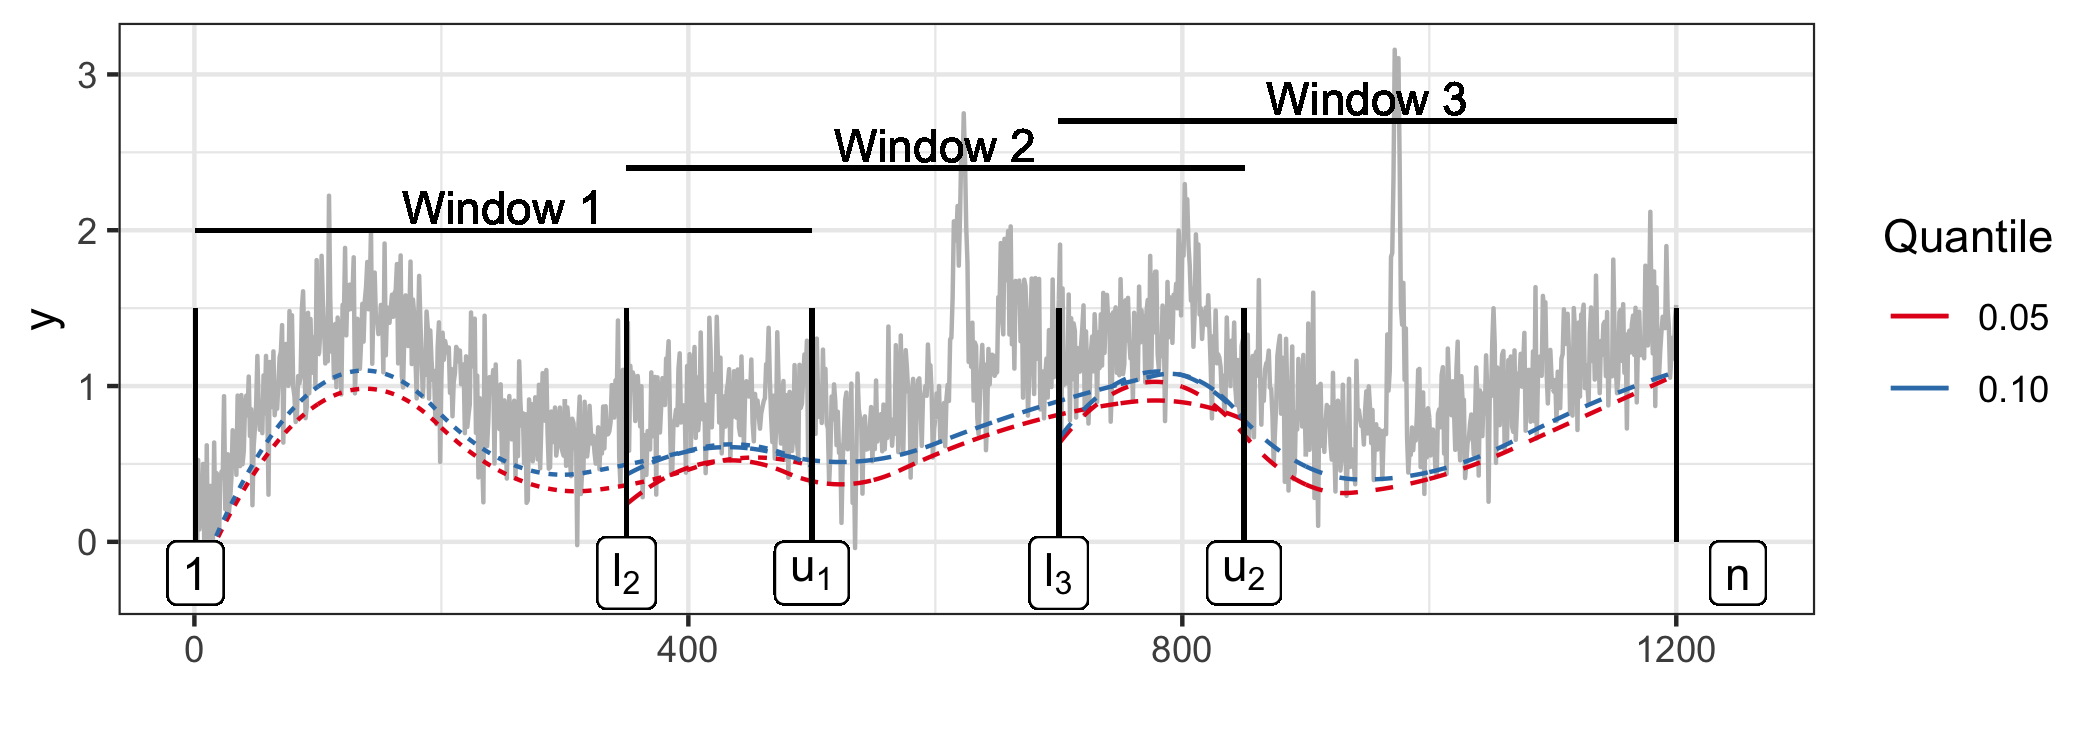
\includegraphics[width = 0.8\linewidth]{Figures/overlapping_windows.png}
	\end{figure}

	\begin{algorithm}
		\caption{ADMM algorithm for quantile trend filtering with windows}\label{euclid}
		\begin{algorithmic}		
			\State Define $D = D^{(k+1)}$. 
			\State \textbf{initialize:} \\
				 $\theta_{j,m}^{(0)} = \arg \min \sum_{j=1}^J\rho_{\tau_j}(y_m - \theta_{j,m})+\lambda \lVert D\theta_{j,m}\rVert_1$ subject to $\theta_{1,m}(t) < ...<\theta_{J,m}(t)$ for all $t$. \\		
			 	 $\omega_{j,m}^{(0)} = \mathbf{0}$	
			\Repeat{}
			\State  		
			$\bar{\theta}_{j,m}^{(q)} = g(\theta_{j, m-1}^{(q-1)}, \theta_{j,m}^{(q-1)}, \theta_{j,m+1}^{(q-1)})$
			\State 
			$\omega_{j,m}^{(q)} = \omega_{j,m}^{(q-1)} + \gamma(\theta_{j,m}^{(q-1)} - \bar{\theta}_{j,m}^{(q)})$	
			\State
				$\theta_{j,m}^{(q)} = \arg\min \mathcal{L}(\theta_{j,m}, \bar{\theta}_{j,m}^{(q-1)}, \omega_{j,m}^{(q-1)})$			
			 subject to $\theta_{1,m}(t) < ...<\theta_{J,m}(t)$ for all $t$.
			\Until {convergence}
			\State \textbf{return} Non-overlapping sequence of $\bar{\theta}_{j,m}^{(q)}$ for all $j$, $m$.
			
		\end{algorithmic}
	\end{algorithm}

	We used the stopping criteria described by \cite{boyd2011distributed}. The criteria are based on the primal and dual residuals which represent the residuals for the primal and dual feasibility, respectively. The primal and dual residuals are defined as 
	
	\begin{align}
	&r_p^{(q)} = \sqrt{\sum_{m=1}^M\sum_{j=1}^J\lVert\theta_{j,m}^{(q)} - \bar{\theta}_{j,m}^{(q)}\rVert_2^2}\\
	&r_d^{(q)} = \gamma\sqrt{\sum_{m=1}^M \sum_{j=1}^J\lVert\bar{\theta}_{j,m}^{(q)} - \bar{\theta}_{j,m}^{(q-1)}\rVert_2^2}.
	\end{align}
	
	The primal residual, $r_p$, represents the difference between the trend values in the windows and the consensus trend value while the dual residual, $r_d$s represents the change in the consensus variable from one iterate to the next. The algorithm is stopped when 
	
	\begin{align}
		&r_p^{(q)} < \epsilon_{abs}\sqrt{NJ} + \epsilon_{rel}\underset{m}{\max}\left[\max 
		\left(\sqrt{\sum_{j=1}^J \lVert\theta_{j,m}^{(q)}\rVert_2^2}, \sqrt{\sum_{j=1}^J \lVert \bar{\theta}_{j,m}^{(q)} \rVert_2^2} \right )\right]\\
		&r_d^{(q)} < \epsilon_{abs}\sqrt{NJ} + \epsilon_{rel}\sqrt{\sum_{m=1}^M\sum_{j=1}^J\lVert \omega_{j,m}^{(q)}\rVert_2^2}
	\end{align}
	

	
	\begin{figure}
		\centering
		\caption{Trend fit with our ADMM algorithm with 3 windows which converged in 7 iterations compared to trend from simultaneous fit.}
		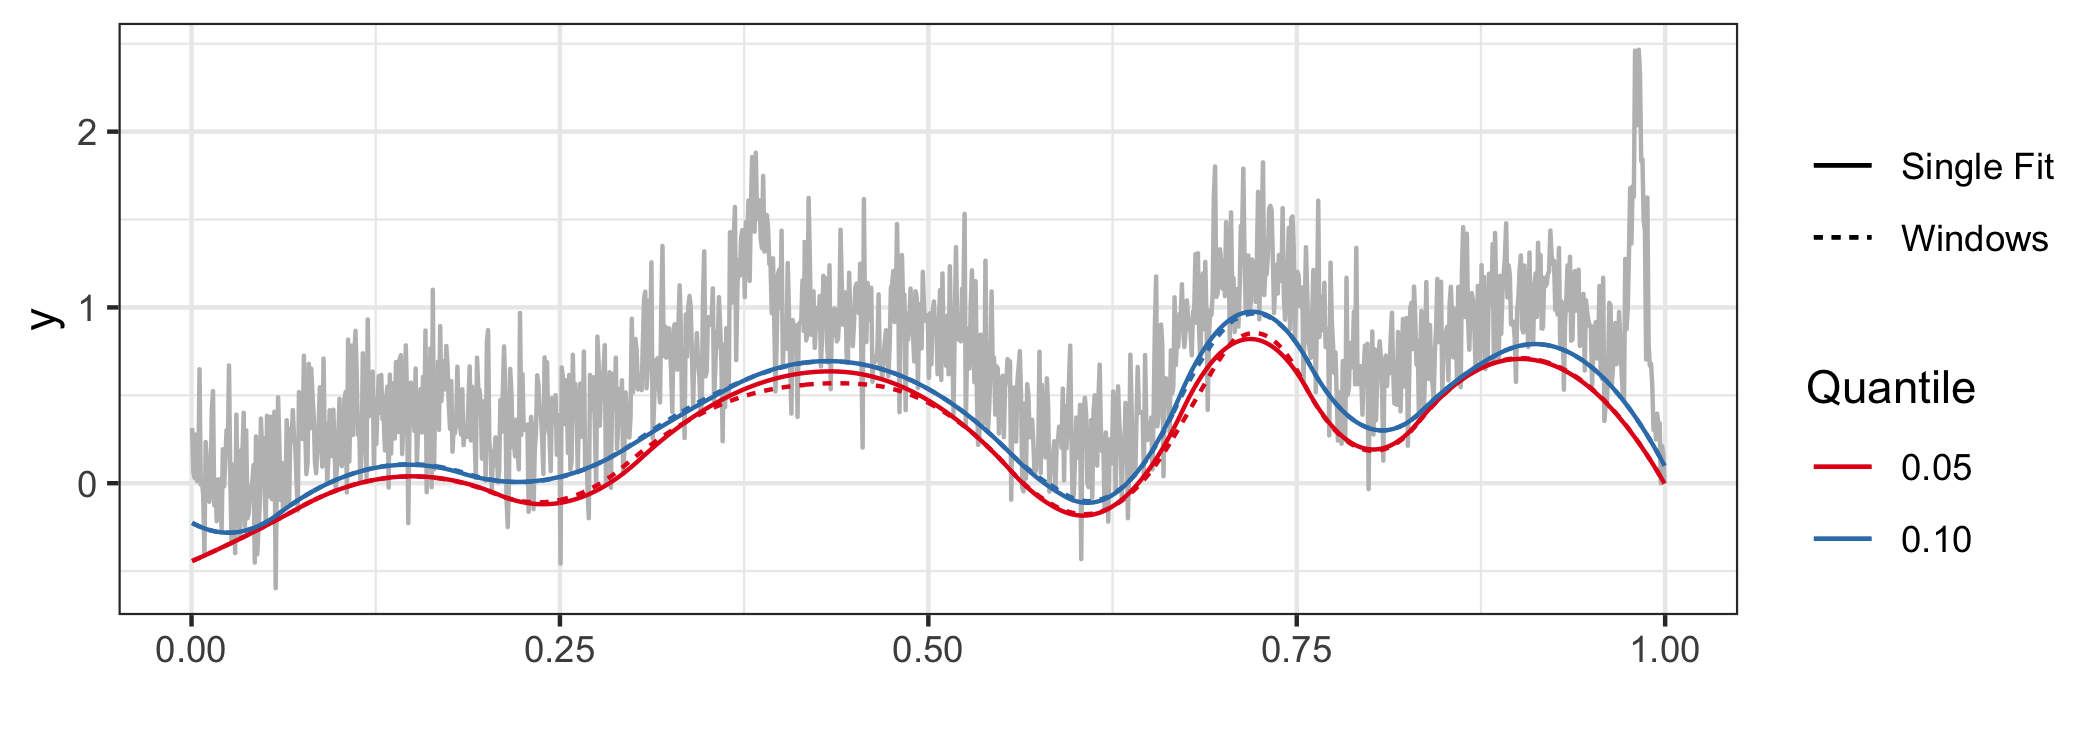
\includegraphics[width = 0.8\linewidth]{Figures/admm_windows.png}
	\end{figure}

	Timing experiments illustrate the advantages of using our ADMM algorithm even on datasets where solving the problem simultaneously is possible. We use from one to four windows for each data size with an overlap of 500. The windows algorithm was run until the stopping criteria were met using $\epsilon_{abs} = 0.01$ and $\epsilon_{rel} = 0.001$. For each data size, $n$, 25 datasets were simulated using the peaks simulation design described below and trends for three quantiles were fit simultaneously: 0.05, 0.1, and 0.15 using a $\lambda = n/5$.
	
	\begin{figure}[!h] 
		\centering
		\caption{Timing experiments comparing quantile trend filtering with varying numbers of windows by data size.}
		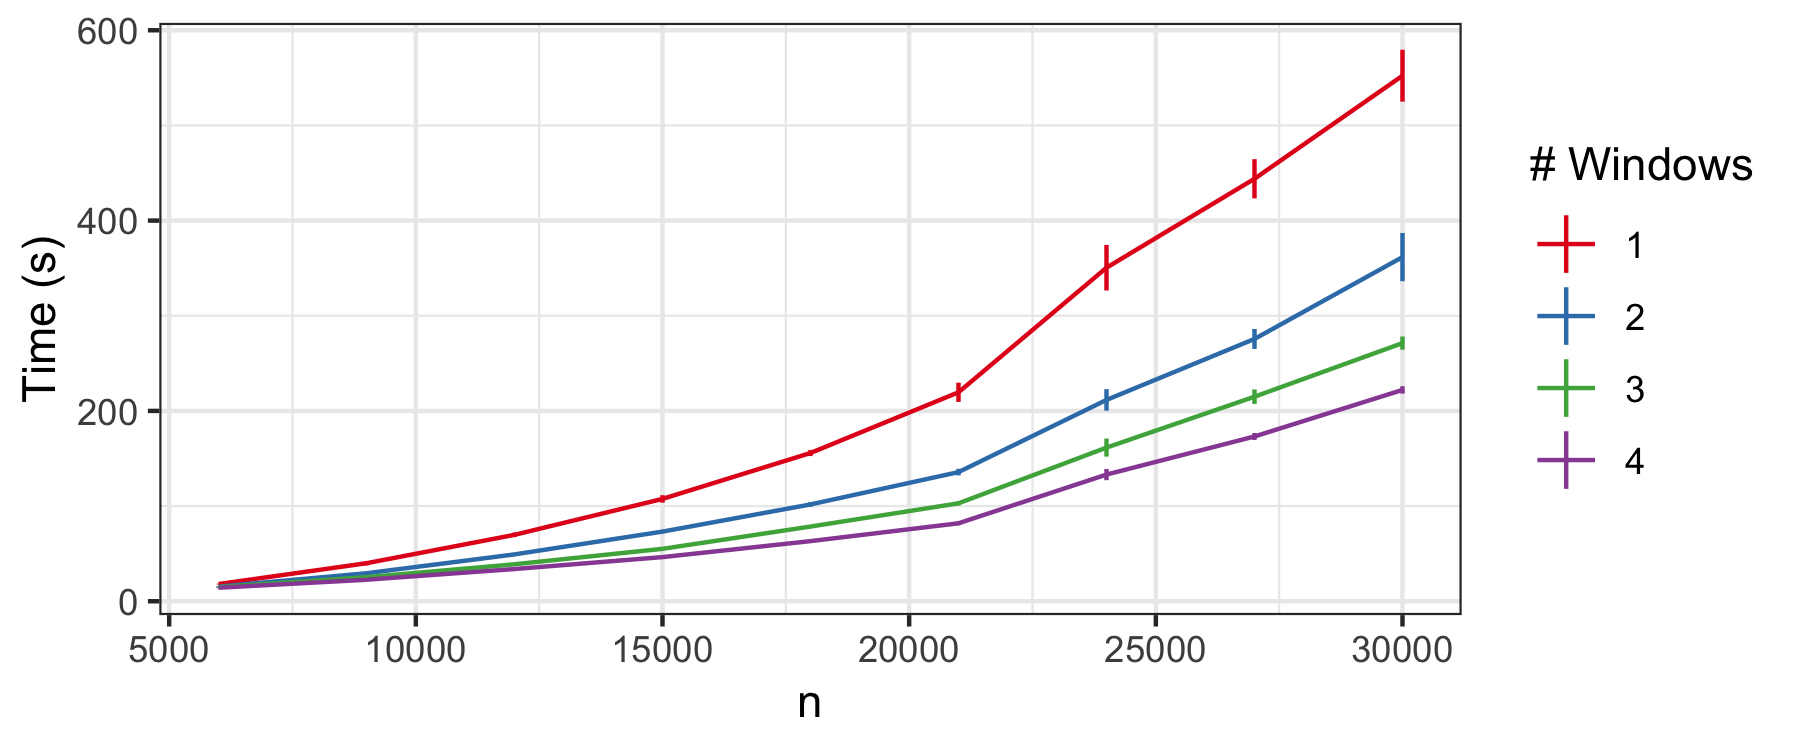
\includegraphics[width = 0.7\linewidth]{Figures/Fig_timing_experiment.png}
	\end{figure}

	\subsection{Regularization Parameter Choice}
	\label{sec:lambda_choice}
	Our method can easily handle missing data by changing the check loss function to output 0 for missing values. This allows us to leave out validation observations that can be used to select the tuning parameter $\lambda$ and to compare method performance on real data. A number of methods have been proposed for selecting the quantile regression smoothing spline tuning parameter \cite{yuan2006gacv}.  \cite{KoenkerNgPortnoy1994} relate $\lambda$ to the number of interpolated points $p_{\lambda} = \sum I(y_i = \widehat{g}_i(x_i))$, which can be thought of as active knots, they propose the Schwarz criterion for the selection of $\lambda$
	\begin{equation}
	\mbox{SIC}(p_{\lambda}) = \log[\frac{1}{n}\rho_{\tau}(y - \widehat{g}(x))] + \frac{1}{2n}p_{\lambda}\log n
	\end{equation}
	
	The traditional Bayesian Information Criterion (BIC) is given by 
	\begin{equation}
	\mbox{BIC}(s) = -2\log(L\{\hat{\theta}(s)\}) + \nu(s)\log n 
	\end{equation}	
	where $\theta(s)$ is the parameter $\theta$ with those components outside $s$ being set to 0, and $\nu(s)$ is the number of components in $s$. If we assume an asymmetric Laplace likelihood $L(y|\theta) = \left(\frac{\tau^n(1-\tau)}{\sigma}\right)^n\exp\left\{-\sum_i\rho_\tau(\frac{y_i - \theta_i}{\sigma})\right\}$ and the number of non-zero elements of $D\theta$ as $df$
	\begin{equation}
	\mbox{BIC}(df) = 2\frac{1}{\sigma}\rho_{\tau}(y-\theta) + \mbox{df}\log n
	\end{equation} 
	We can choose any $\sigma>0$ and have found empirically that $\sigma =  \frac{1-|1-2\tau|}{2}$ produces stable estimates. \cite{chen2008} proposed the extended BIC for large parameter spaces 
	\begin{equation}
	\mbox{BIC}_{\gamma}(s) = -2\log(L\{\hat{\theta}(s)\}) + \nu(s)\log n  + 2\gamma\log{P\choose j,}~~\gamma \in [0,1]
	\end{equation}
	where $P$ is the total number of possible parameters and $j$ is the number of parameters included in given model. We used this criteria with $\gamma = 1$, $P=n-k$ where $k$ is the order of the differencing matrix and $j = \nu(s)$ is the number of non-zero entries in $D^{(k)}\theta$. 
	
	We used a single dataset to illustrate the difference between the scaled, unscaled and extended BIC criteria. 
	
	\begin{figure}[h!]
		\caption{Degrees of freedom (number of non-zero elements of $D\theta$) by $\log(\lambda)$.} 
		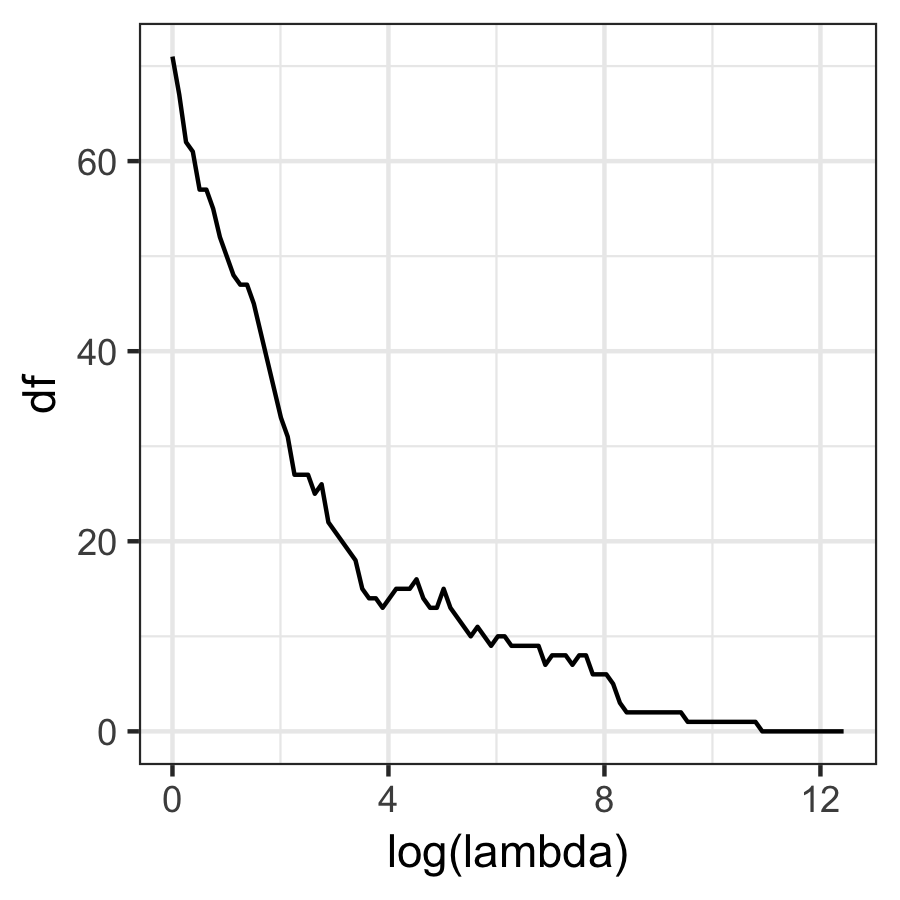
\includegraphics[width = 0.25\linewidth]{Figures/df_by_lambda.png}
		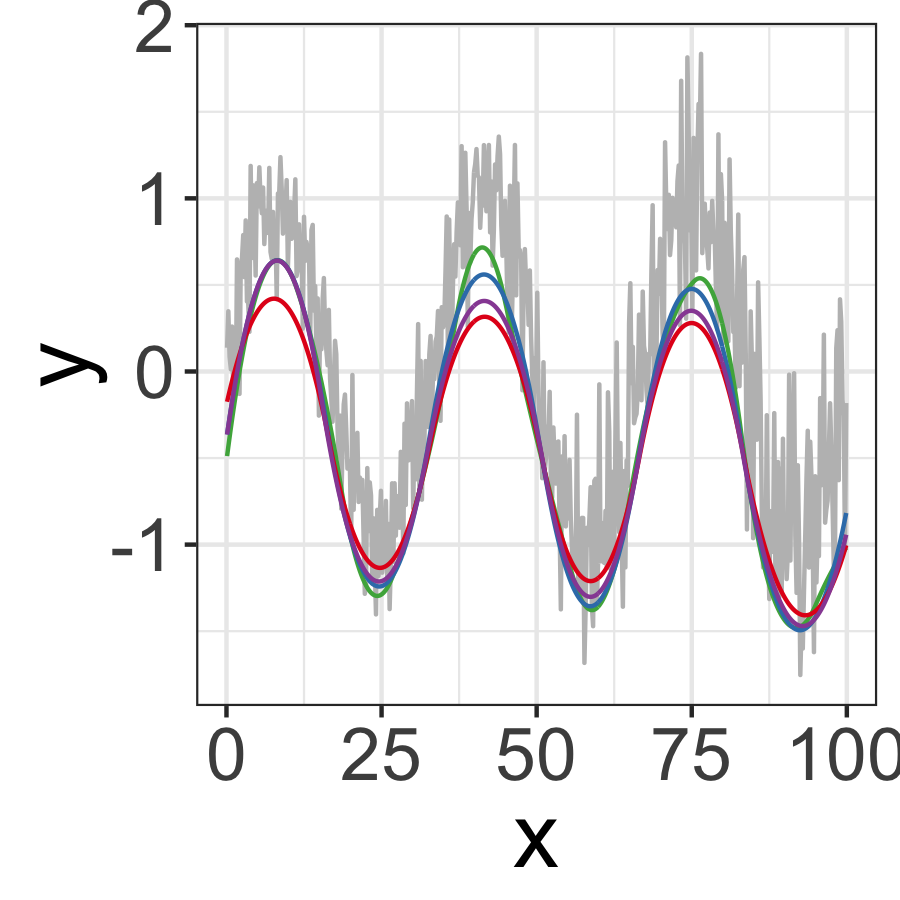
\includegraphics[width = 0.25\linewidth]{Figures/BIC_data.png}
		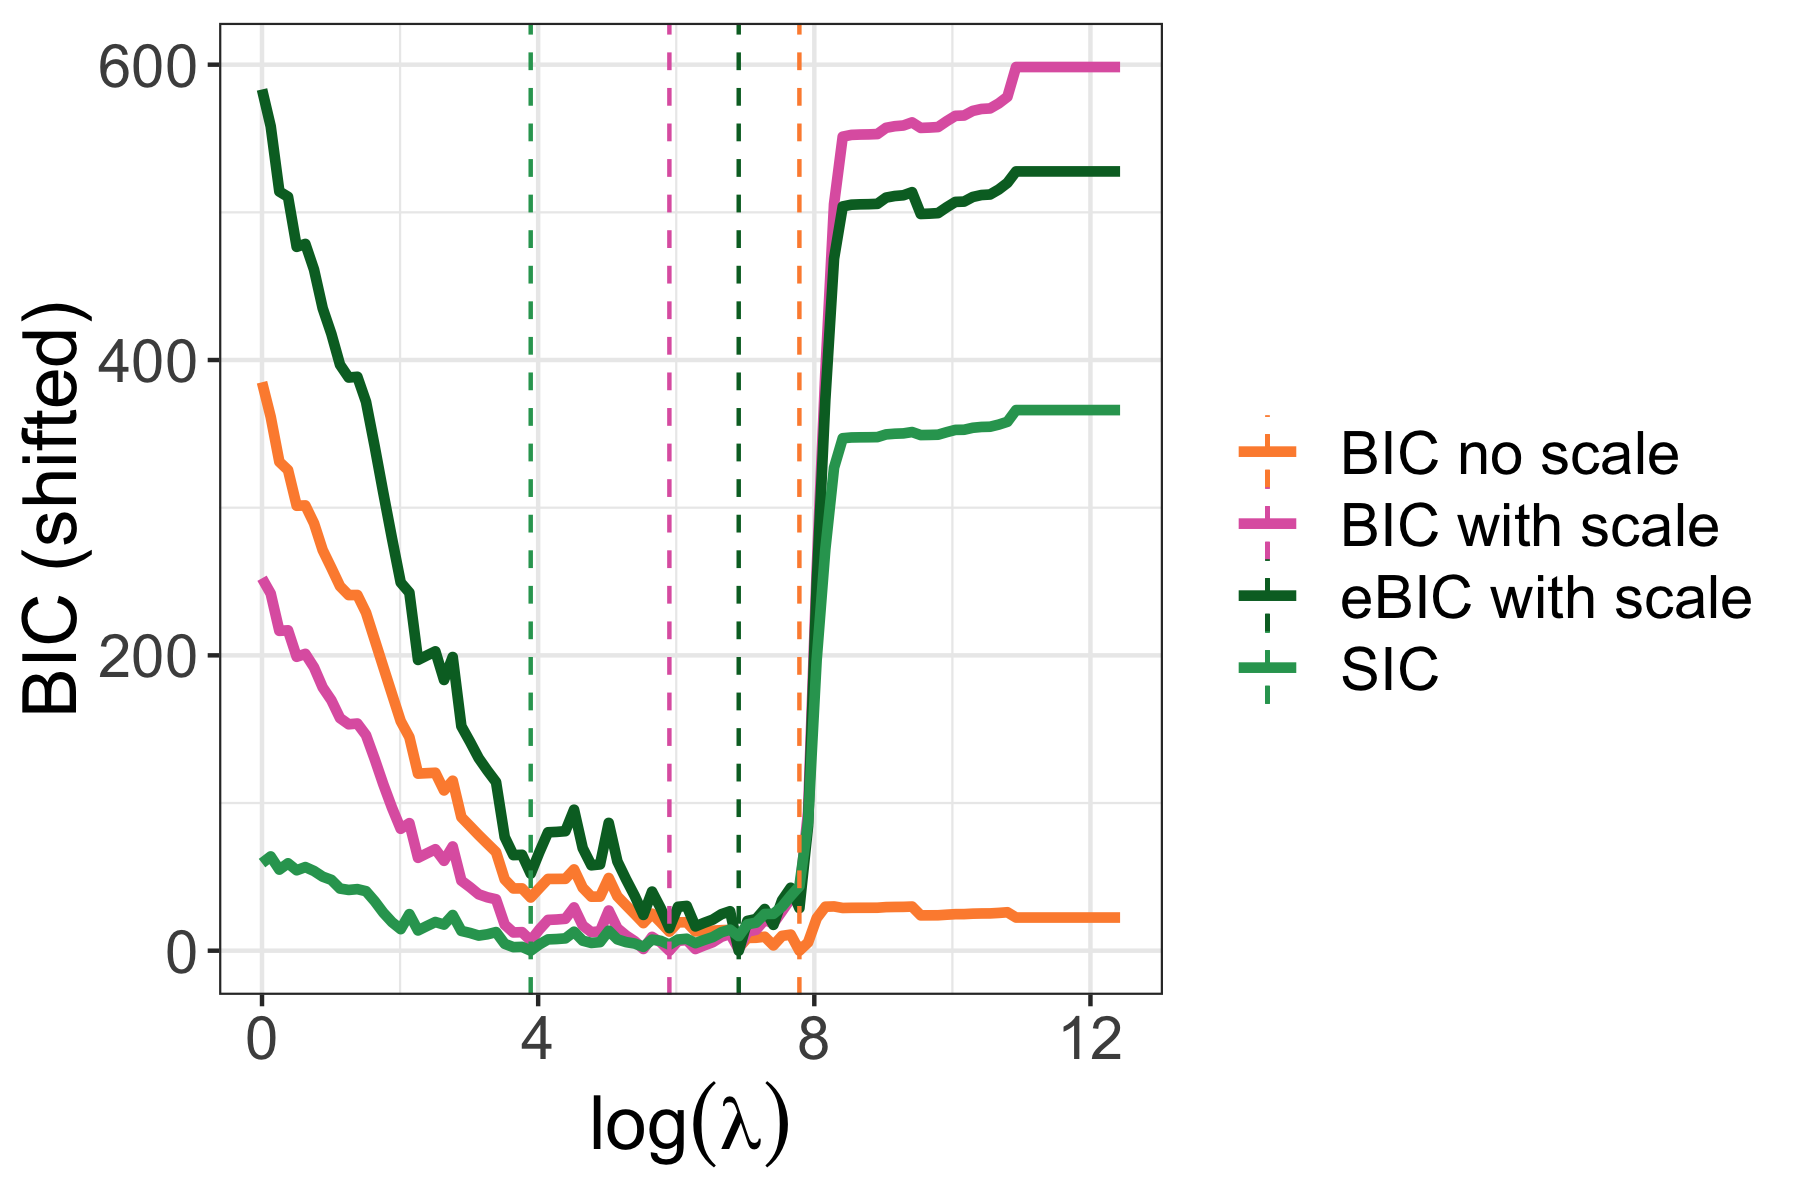
\includegraphics[width = 0.5\linewidth]{Figures/BIC_by_lambda.png}
	\end{figure}

	\section{Simulation Studies}
	
	\subsection{Estimating Quantiles}
	
	We compare the performance of our quantile trend filtering method with the three previously published methods using designs proposed by \cite{Racine2017}. The methods compared are: \texttt{npqw} which is the quantile-ll method described in \cite{Racine2017}, code was obtained from the author; \texttt{qsreg} in the \texttt{fields} R package and described in \cite{Oh2011}; \texttt{rqss} available in the \texttt{quantreg} package and described in \cite{KoenkerNgPortnoy1994}.  The smoothing parameter $\lambda$ for the \texttt{rqss} method is chosen using a grid search and minimizing the SIC criteria as described in \cite{KoenkerNgPortnoy1994}. We further compare three criteria for choosing the smoothing parameter for our detrend method: \texttt{detrendr\_SIC}: Our method where we minimize $\sum_i\rho_{\tau}(y_i - \theta_i) + \lambda||D\theta||_1$ and $\lambda$ is chosen using SIC \citep{KoenkerNgPortnoy1994}.  \texttt{detrendr\_valid}: Our method where lambda is chosen by leaving out every 5th observation as a validation data set and minimizing the evaluating the check loss function evaluated at the validation data. \texttt{detrendr\_eBIC}:  the new criteria we have proposed based on the extended BIC proposed by \cite{chen2008}. 
	 
	Three simulation designs from \cite{Racine2017} were considered. For all designs $X_i$ was generated as a uniformly spaced sequence in $[0,1]$ and the response $Y$ was generated as 
	$$Y_i = sin(2\pi x_i) + \epsilon_i(x_i)$$
	The three error distributions considered were 
	\begin{itemize}
		\item Gaussian: $\epsilon_i(x_i) \sim N\left(0, \left(\frac{1+x_i^2}{4}\right)^2\right)$
		\item Beta: $\epsilon_i \sim Beta(1, 11-10x_i)$
		\item Mixed normal: $\epsilon_i$ is simulated from a mixture of $N(-1,1)$ and  $N(1,1)$ with mixing probability $x_i$.
	\end{itemize}
	\begin{figure}
		\caption{Simulated data with true quantiles $\tau \in \{0.01, 0.05, 0.25, 0.5, .75, 0.95, 0.99\}$}	
		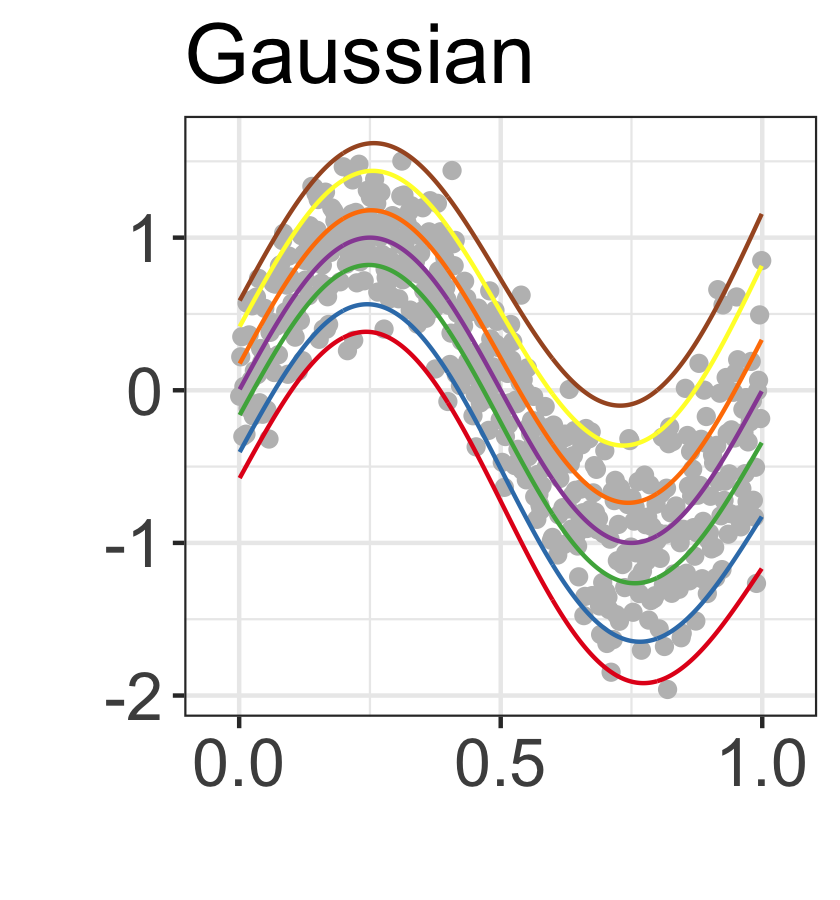
\includegraphics[width=.28\linewidth]{Figures/gaus.png}
		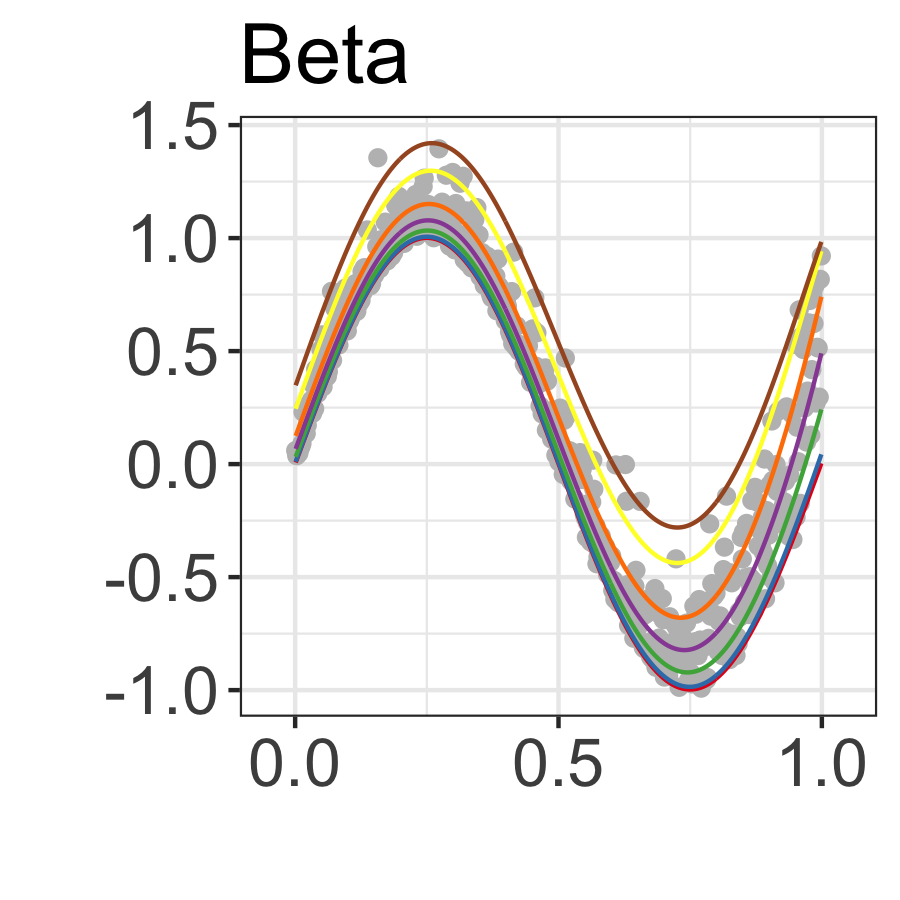
\includegraphics[width=.3\linewidth]{Figures/shapebeta.png}
		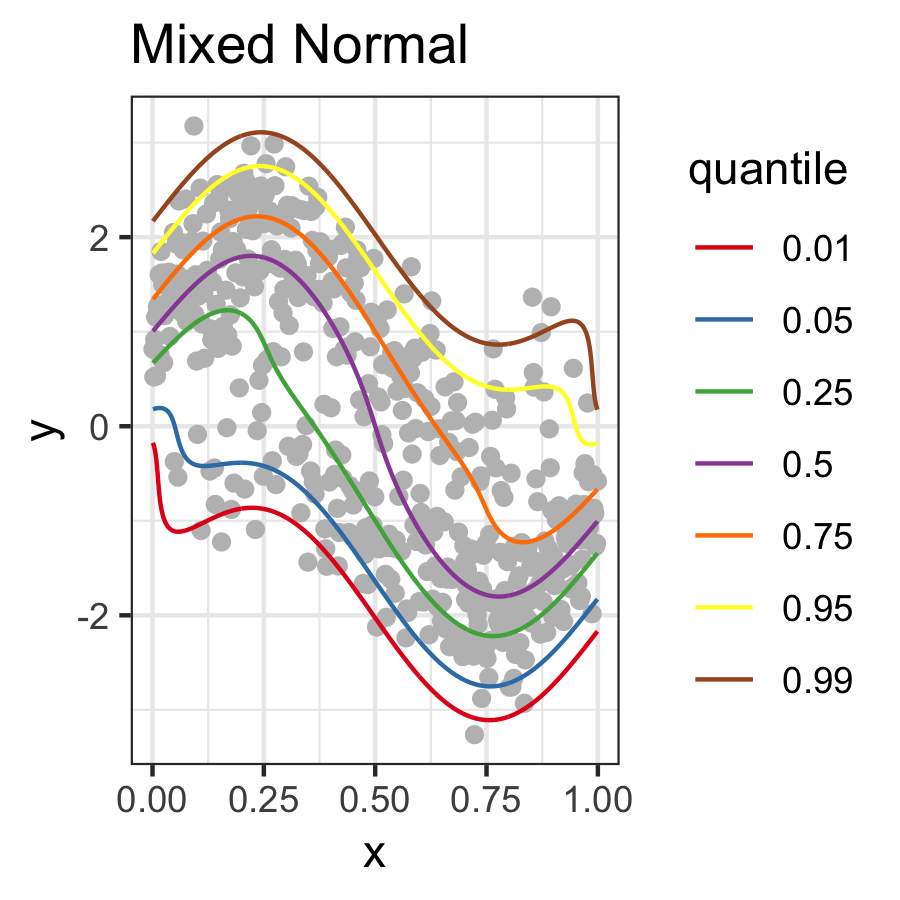
\includegraphics[width=.45\linewidth]{Figures/mixednorm.png}
	\end{figure}
	
	100 datasets were generated of sizes 300, 500 and 1000. The MSE was calculated as $\frac{1}{n}\sum_i (\hat{q}_{\tau}(x_i) - q_\tau(x_i))^2$. The plots below show the mean MSE $\pm$ twice the standard error by method, quantile level and sample size. 
	
	\begin{figure}
		\caption{RMSE by design, method, quantile and data size.}
		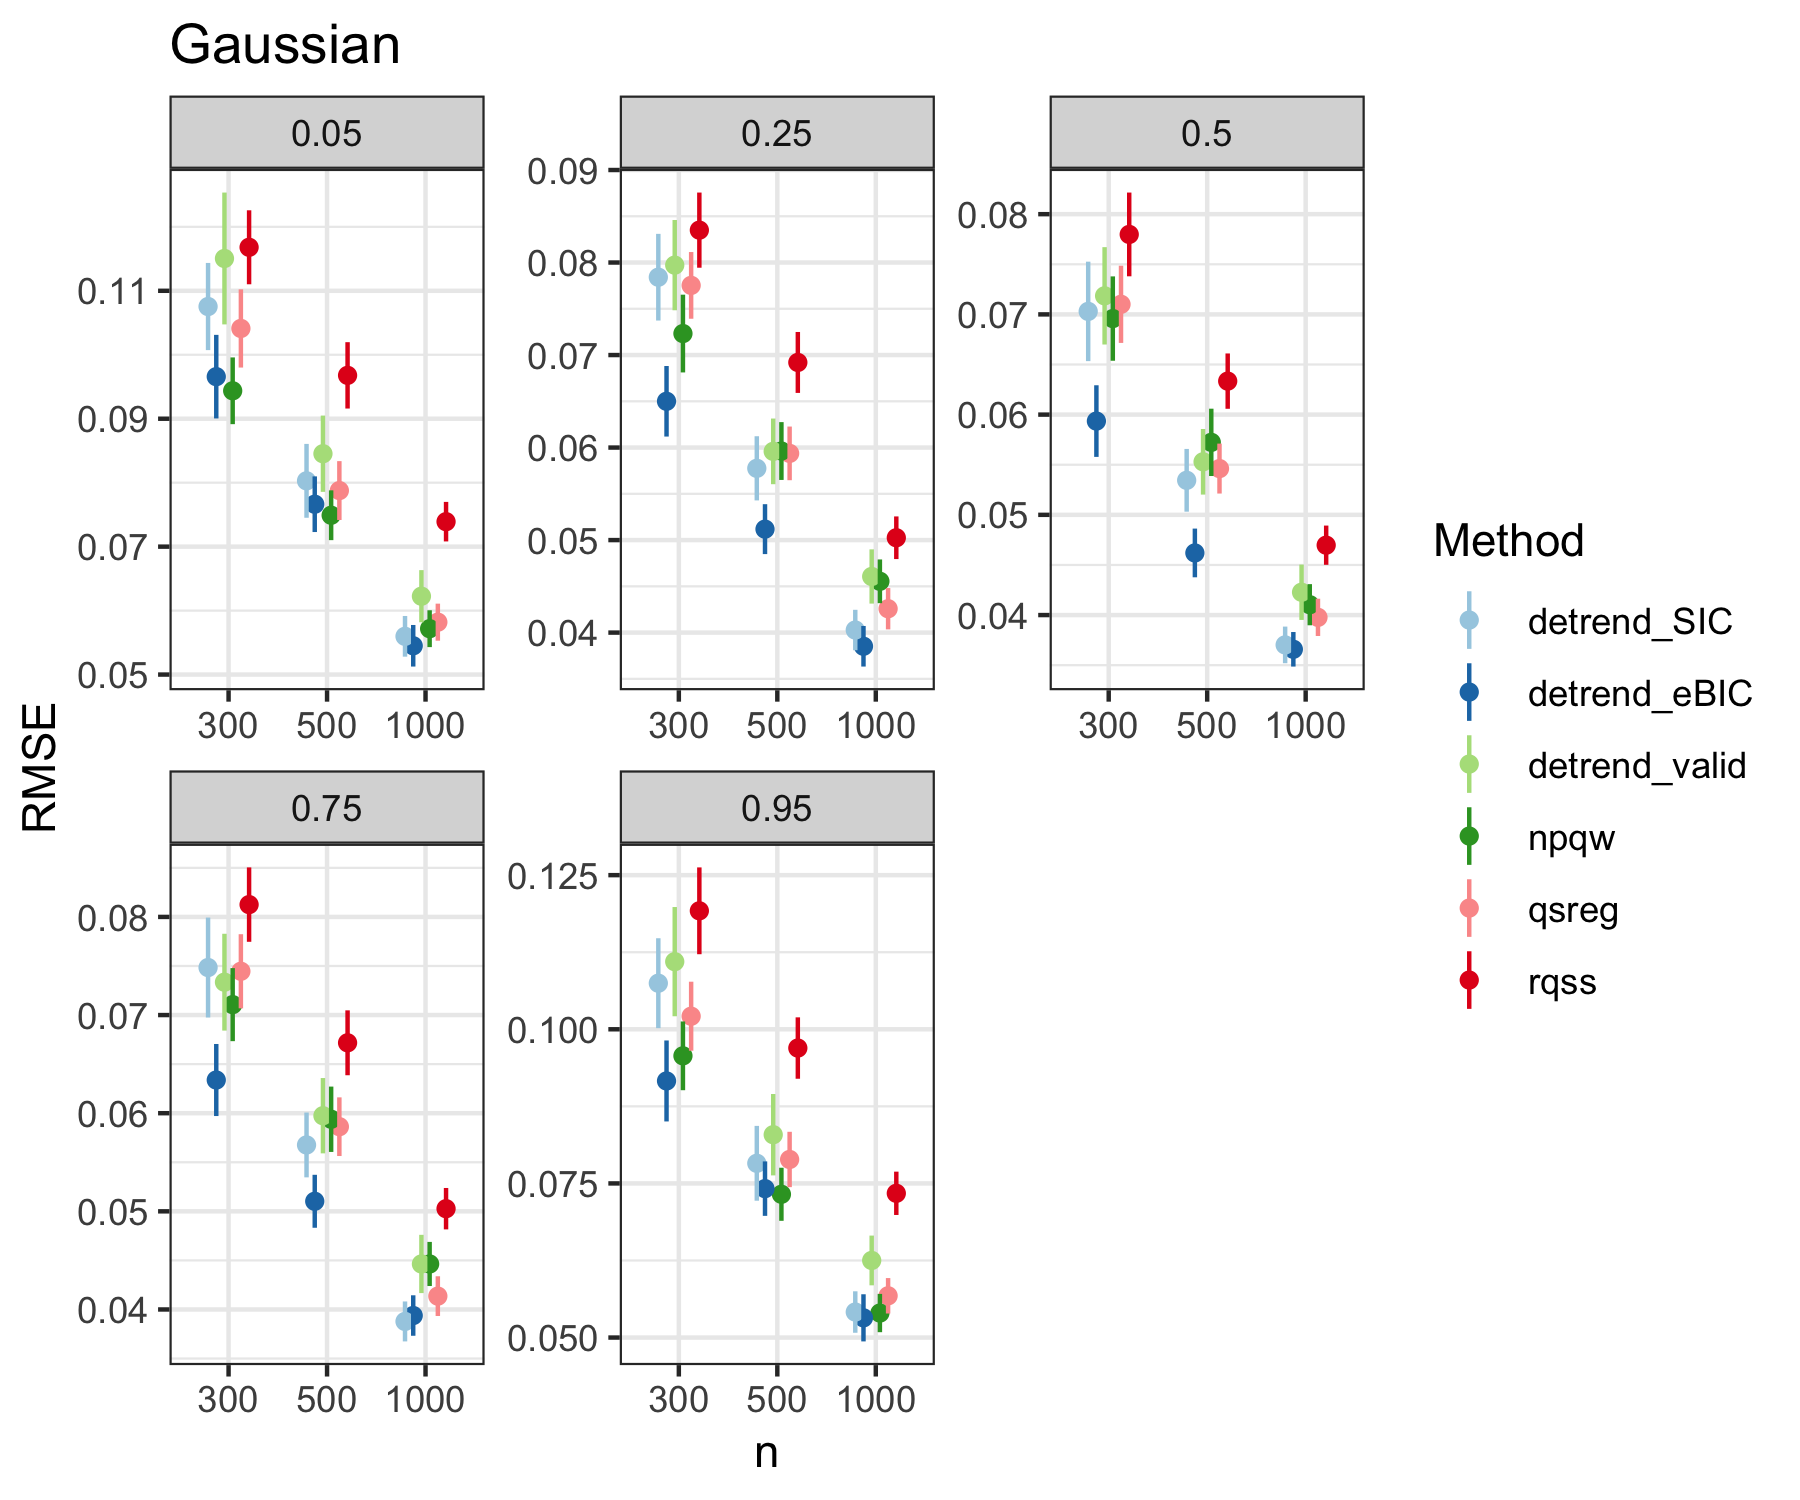
\includegraphics[width=\linewidth]{Figures/gaus_mse.png}	
		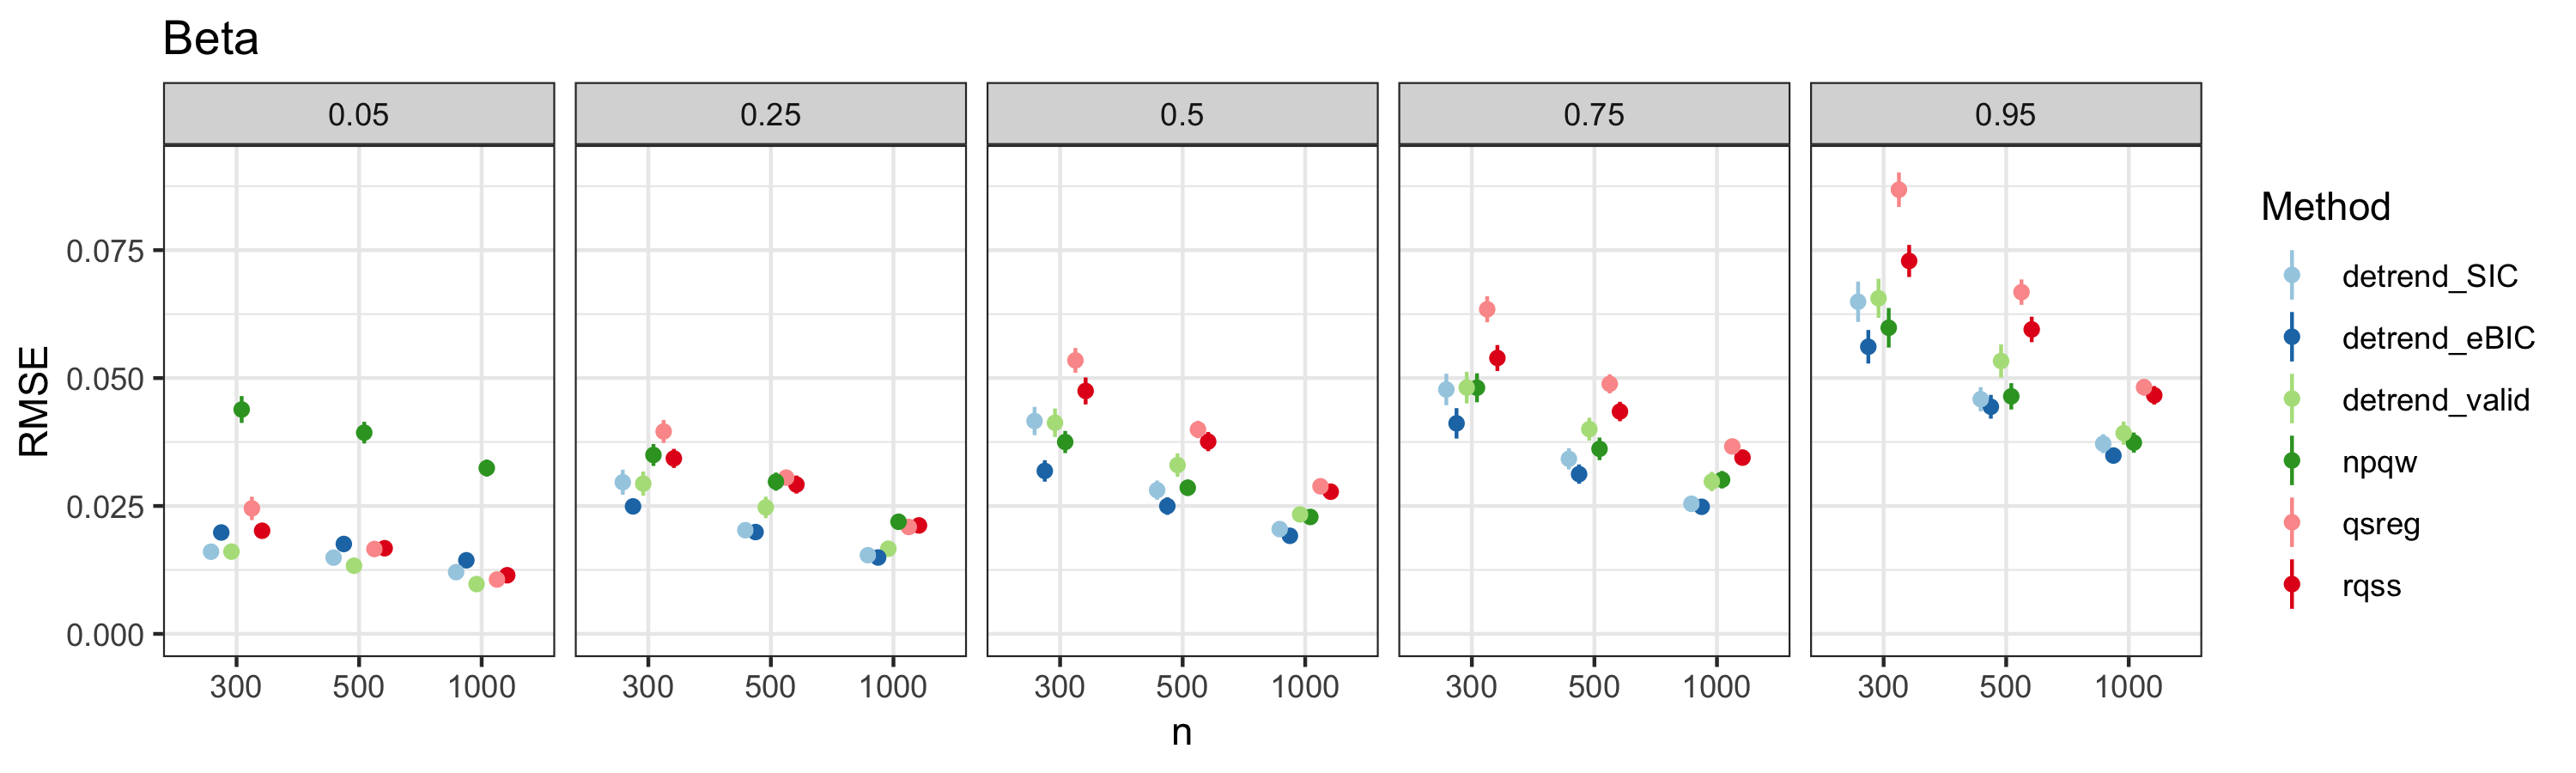
\includegraphics[width=\linewidth]{Figures/shapebeta_mse.png}
		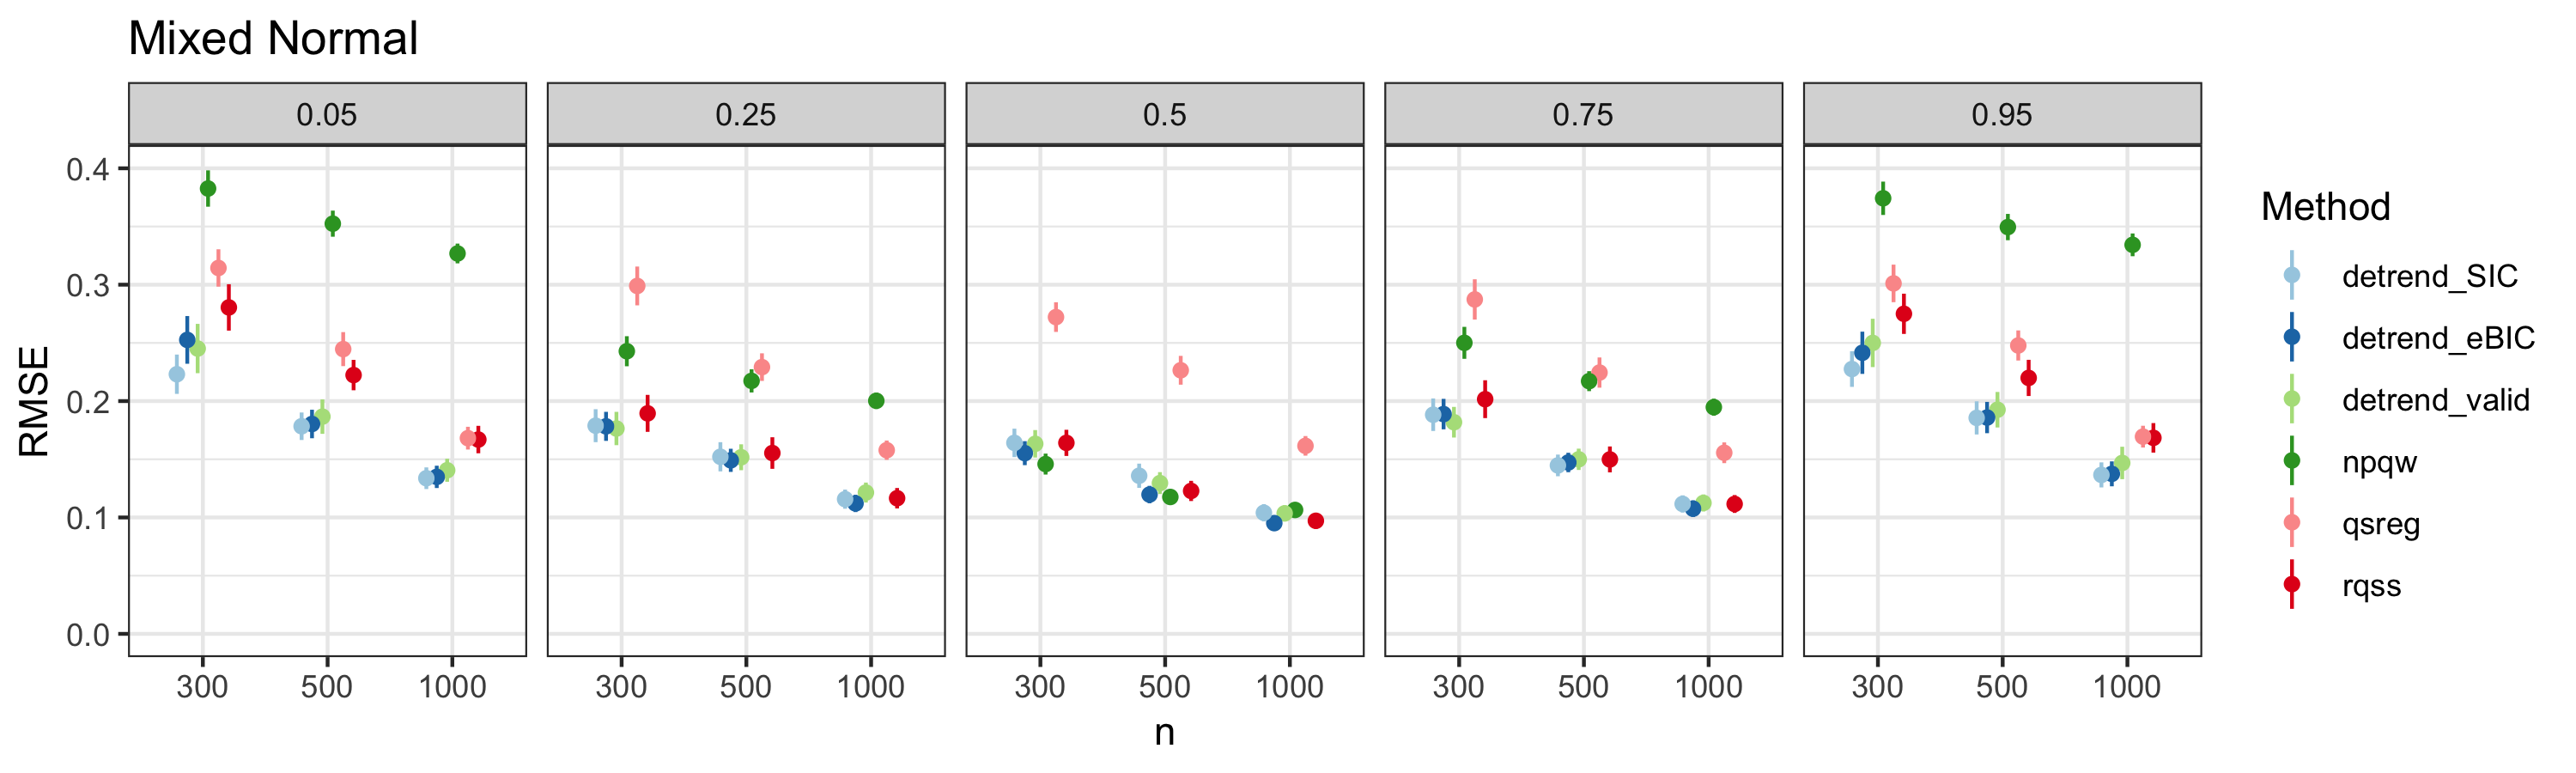
\includegraphics[width=\linewidth]{Figures/mixednorm_mse.png}
	\end{figure}
	In all of the designs the proposed detrend methods are either better than or comparable to existing methods. The npqw method performs particularly poorly in the mixed normal design, due to the fact that it assumes the data comes from a scale-location model which is violated in this case. 
	
	\subsection{Peak Detection}
	\begin{figure}[h]
		\caption{Example of simulated peaks, baseline, and observed measurements.}
		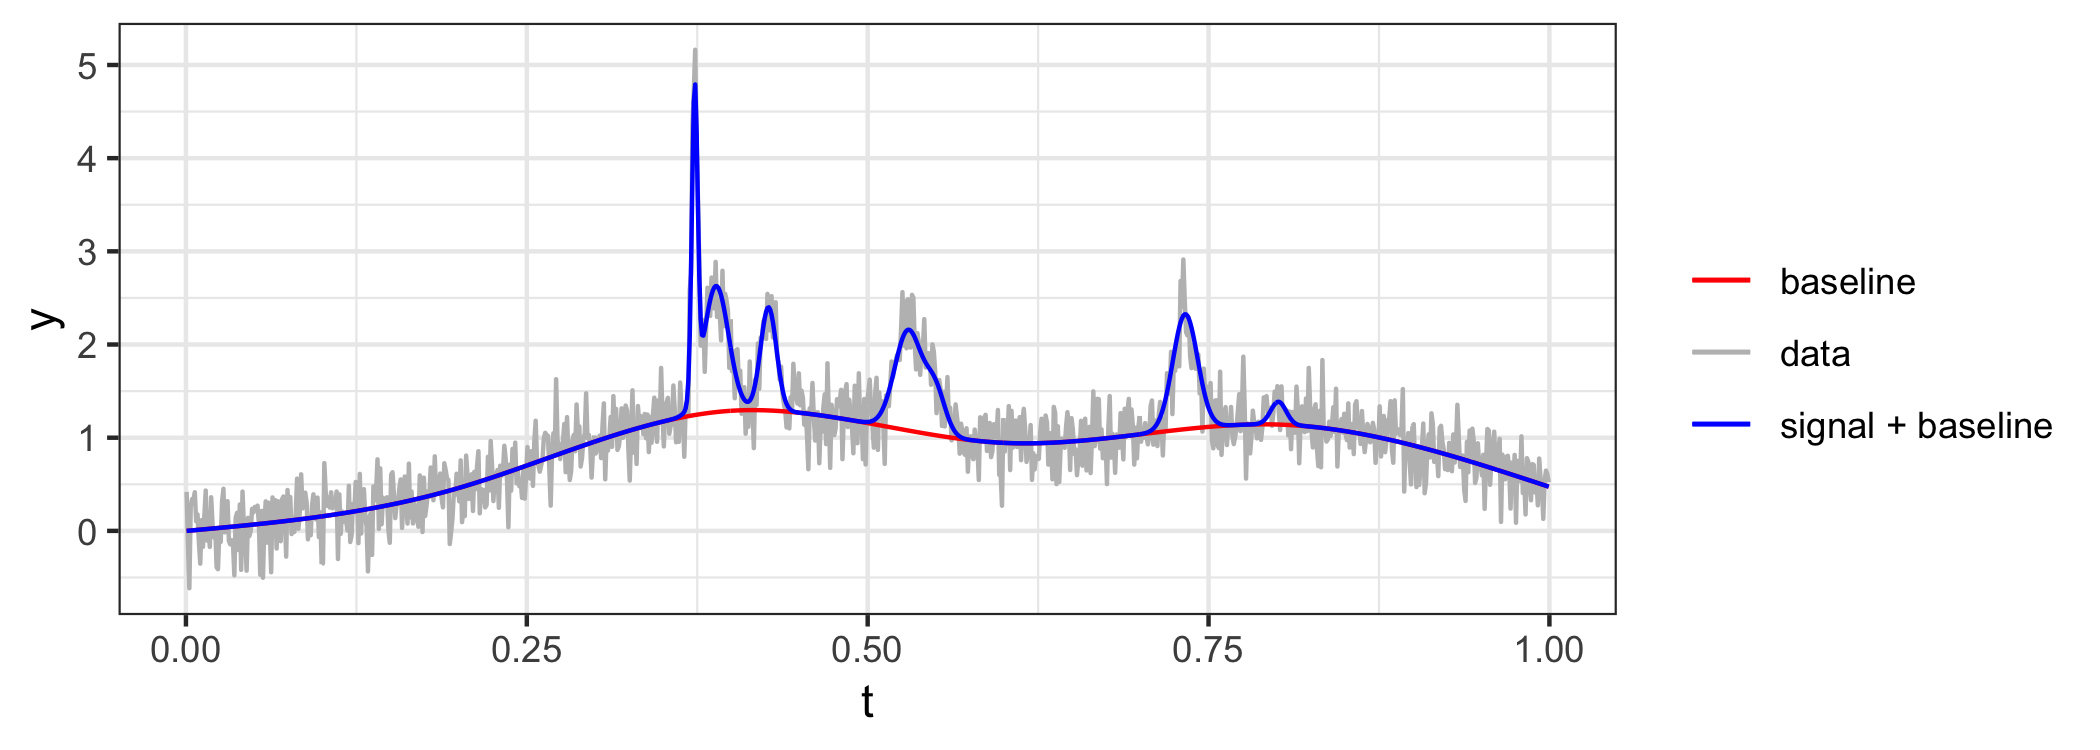
\includegraphics[width = \linewidth]{Figures/ex_peaks.png}
	\end{figure}

	We use another simulation design based on the applied problem we aim to solve. We assume that the measured data can be represented by 
	\begin{equation}
	Y(t) = s(t) + b(t) + \epsilon(t)
	\end{equation} 
	with $t = 1, ..., n$, where $s(t)$ is the true signal at time $t$, $b(t)$ is the drift component that varies smoothly over time and $\epsilon(t) \sim N(0, \sigma^2)$ is an error component. We generate $b(t)$ using a cubic natural spline basis function with degrees of freedom sampled from a Poisson distribution with mean parameter equal to $n/100$,  and coefficients drawn from an exponential distribution with rate 1. The true signal function is assumed to be zero with peaks generated using the Gaussian density function. The number of peaks is sampled from a binomial distribution with size equal to $n$ and probability equal to $0.005$ with location parameters uniformly distributed between $1$ and $n-1$ and bandwidths uniformly distributed between $2$ and $12$. The peaks were then multiplied by a factor that was randomly drawn from a normal distribution with mean 20 and standard deviation of 4. One hundred datasets were generated for $n=\{500, 1000, 2000, 4000\}$. We compare the ability of the methods to estimate the true quantiles of $b(t) + \epsilon$  for $\tau \in \{0.01, 0.05, 0.1\}$ and calculate the RMSE (Fig. \ref{fig:peaks_rmse}). 	
	\begin{figure}
		\caption{RMSE by method, quantile and data size for peaks design.}
		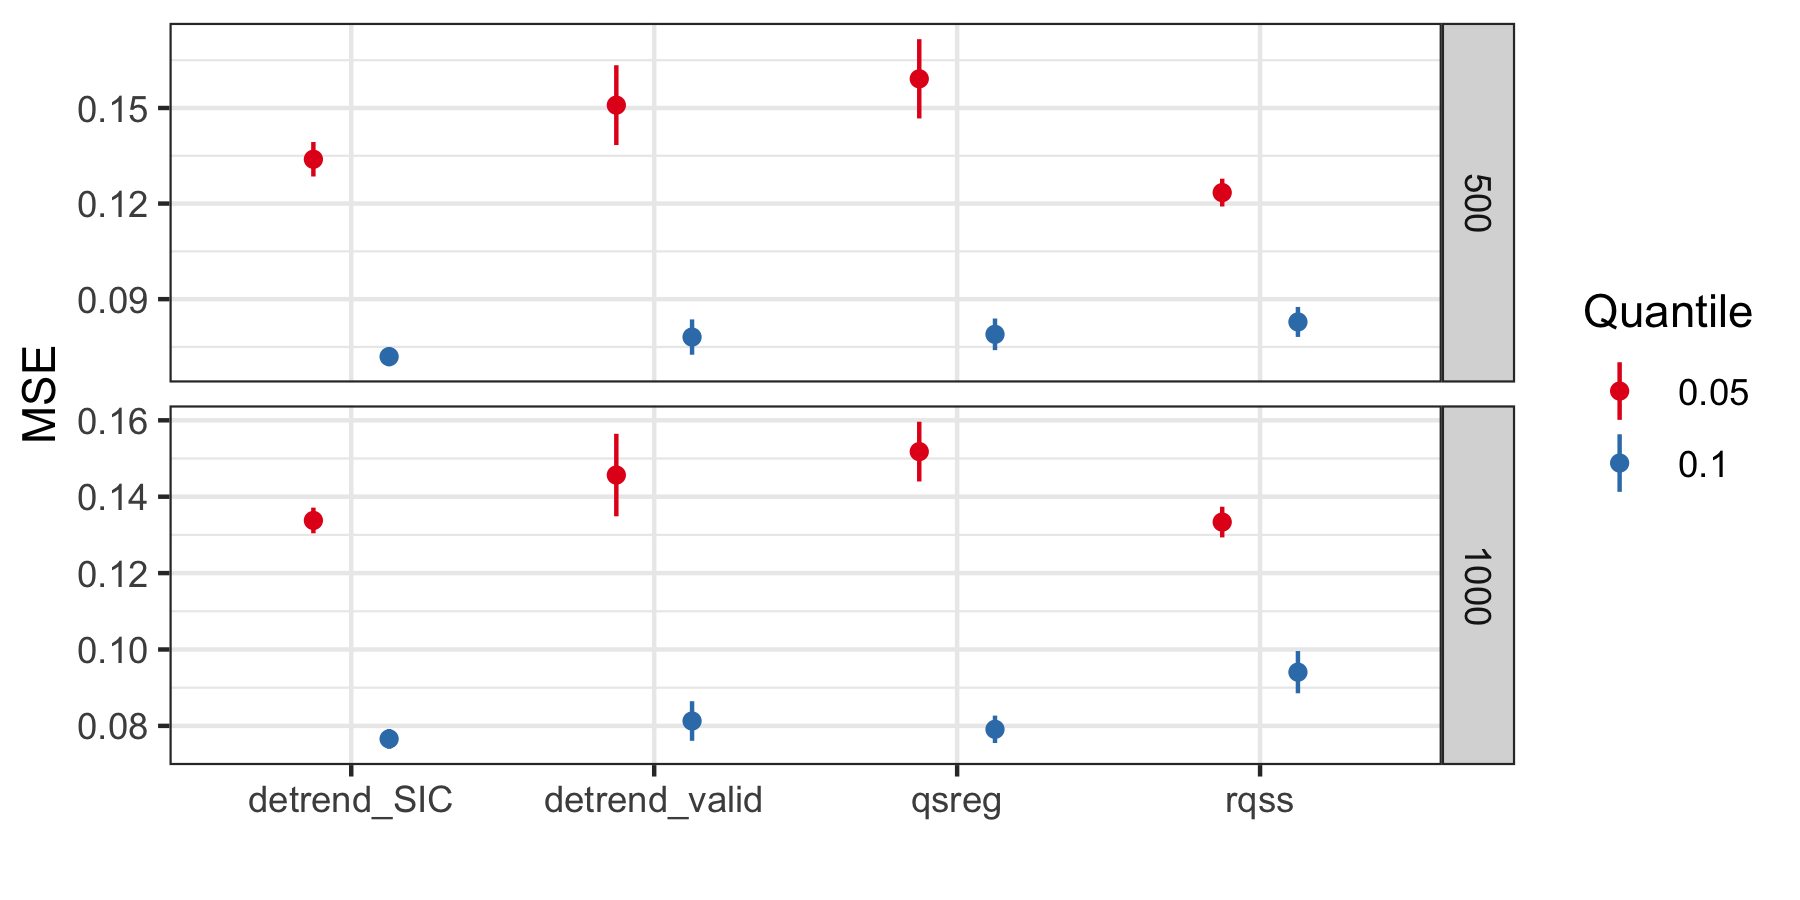
\includegraphics[width = \linewidth]{Figures/peaks_mse.png}	
		\label{fig:peaks_rmse}
	\end{figure}
	
	In our application, we want to accurately classify the observations into signal and no signal using a threshold. To evaluate the accuracy of our method compared to other methods we define true signal as any time when the simulated peak value is greater than 0.5. We compared three different trends for the baseline estimation and four different thresholds for separating the estimated signal after subtracting the estimated baseline from the observations.  An illustration of the observations classified as signal after detrending compared to the ``true signal" is shown in Fig. \ref{fig:peaks_class_eg}.  To compare the resulting signal classifications we calculate the class averaged accuracy (CAA). Defining $s(t) \in \{0,1\}$ as the true vector of signal classification and $\hat{s}(t) \in \{0,1\}$ as the estimated signal classification, the CAA is defined as
	\begin{equation}
	\mbox{CAA} = \frac{1}{2}\left(\frac{\sum_{t=1}^n \mathbf{I}[s(t) = 1 \cap \hat{s}(t)=1]}{\sum_{t=1}^n \mathbf{I}[s(t) = 1]} + \frac{\sum_{t=1}^n \mathbf{I}[s(t) = 0 \cap \hat{s}(t)=0]}{\sum_{t=1}^n \mathbf{I}[s(t) = 0]}\right).
	\end{equation}  
	We use this metric because our classes tend to be very un-balanced in this case with many more $0$s than $1$s. The CAA metric will always give a score of 0.5 for random guessing and also for trivial classifiers such as $\hat{s}(t) = 0$ for all $t$. 

	Our detrend\_BIC method performs the best overall in terms of both RMSE and miss-classification rate. The lowest miss-classification rates were obtained using the detrend\_eBIC method and a threshold of 1 for all data sizes. While qsreg was competitive with our method in some cases, both the RMSE and miss-classification rate increased substantially with the size of the dataset. 
	
	\begin{figure}[h!]
		\caption{Example signal classification using threshold. Red indicates true signal $>0.5$, blue indicates observations classified as signal after baseline removal using eBIC detrendr and a threshold of 1.2.}
		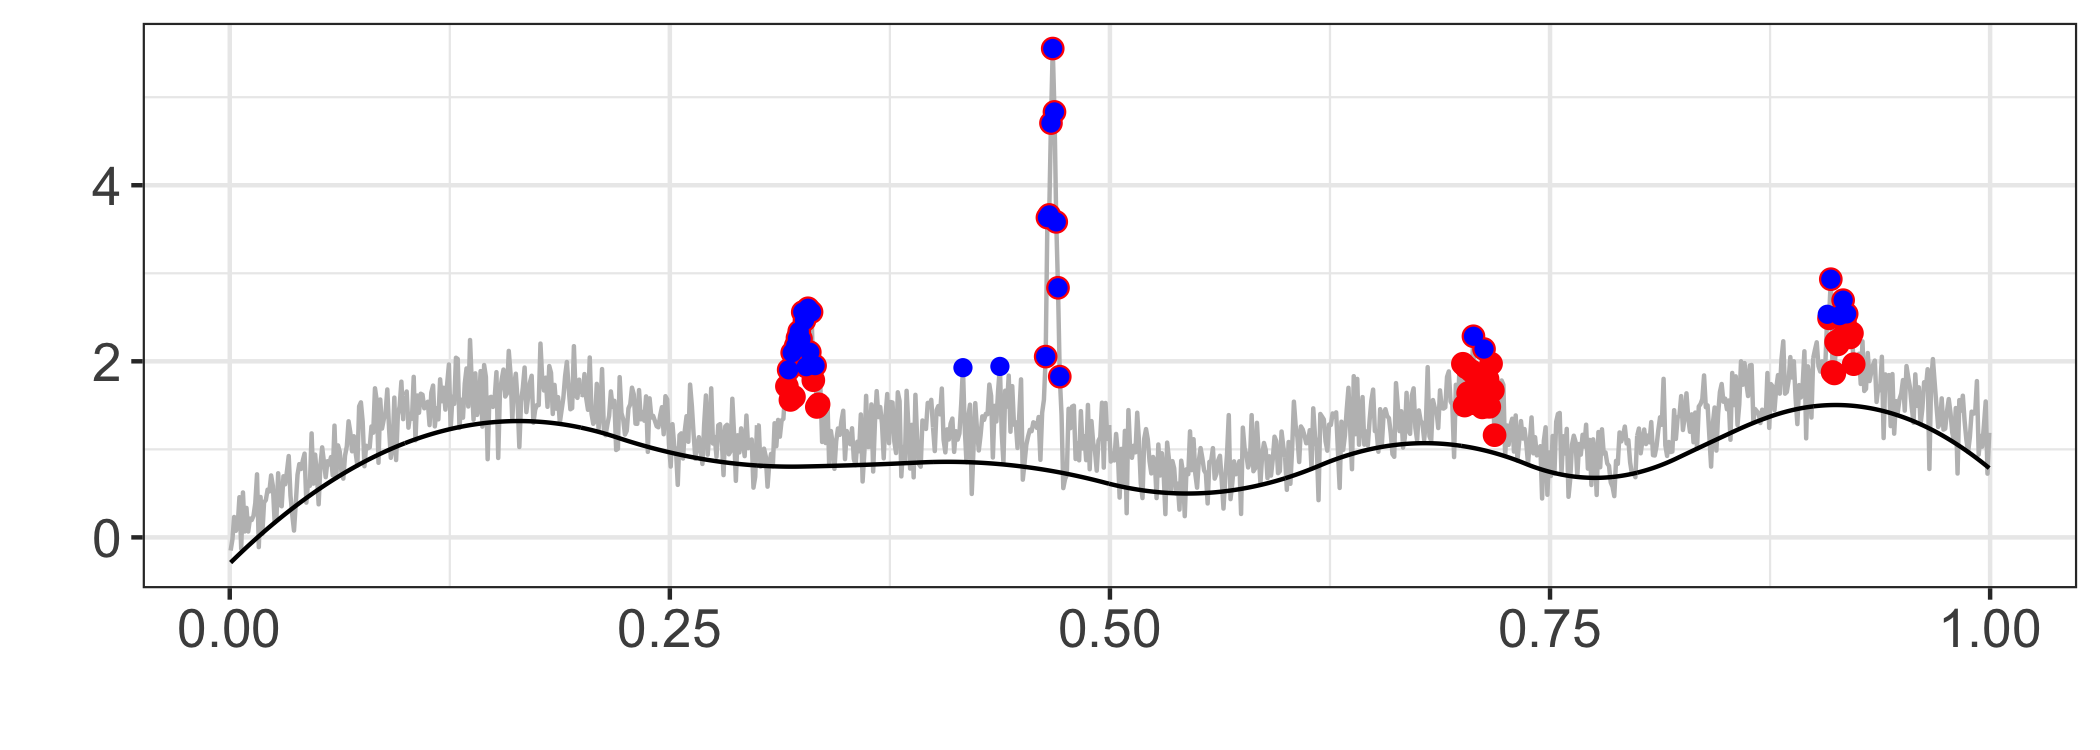
\includegraphics[width = \linewidth]{Figures/peaks_eg_class.png}
		\label{fig:peaks_class_eg}
	\end{figure}
	

	\begin{figure}[h!]
		\caption{Class averaged accuracy by threshold, data size, and method (1 is best 0.5 is worst).}
		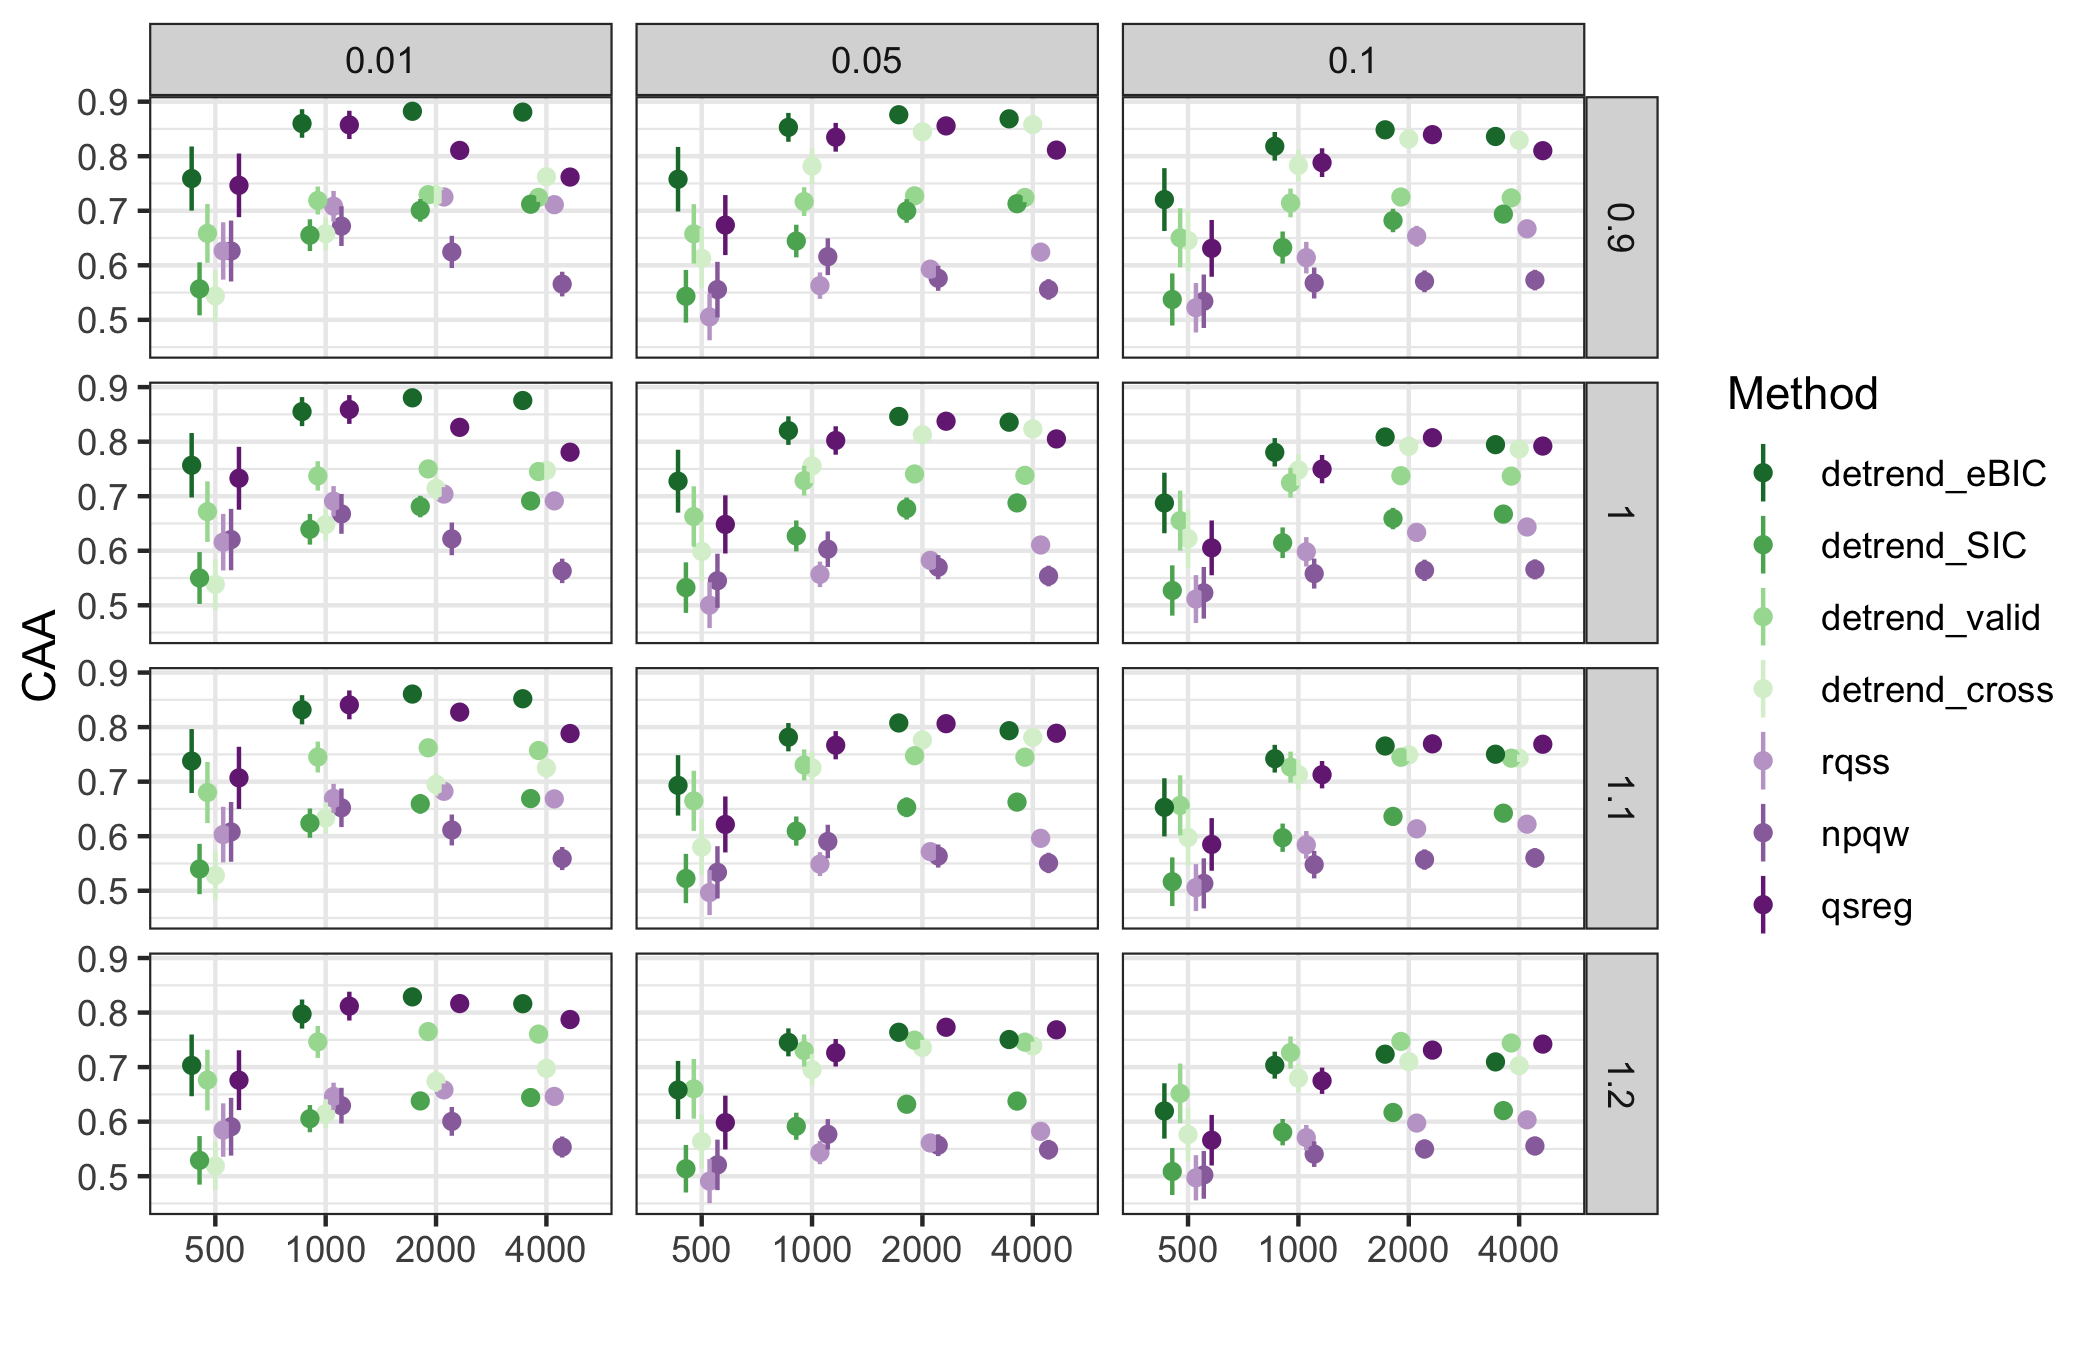
\includegraphics[width = \linewidth]{Figures/peaks_CAA.png}
	\end{figure}


	\FloatBarrier
	
	\section{Application}
	
	We compared our detrend method with the eBIC criteria with the qsreg method on a subset of the real data since the qsreg method cannot handle all 15 hours simultaneously. We estimate the baseline trend using both the 5\textsuperscript{th}, 10\textsuperscript{th}, and 15\textsuperscript{th} quantiles. We compare three thresholds for separating signal from not signal, the thresholds are calculated using the median and a factor multiple of the median absolute deviation of the detrended series. We report both the confusion matrices and the variation of information (VI) distances. 
	

	
		\begin{figure}
		\centering
		\caption{Variation of Information between sensor nodes after trend removal by quantile and method and thresholding by factor of MAD.}
		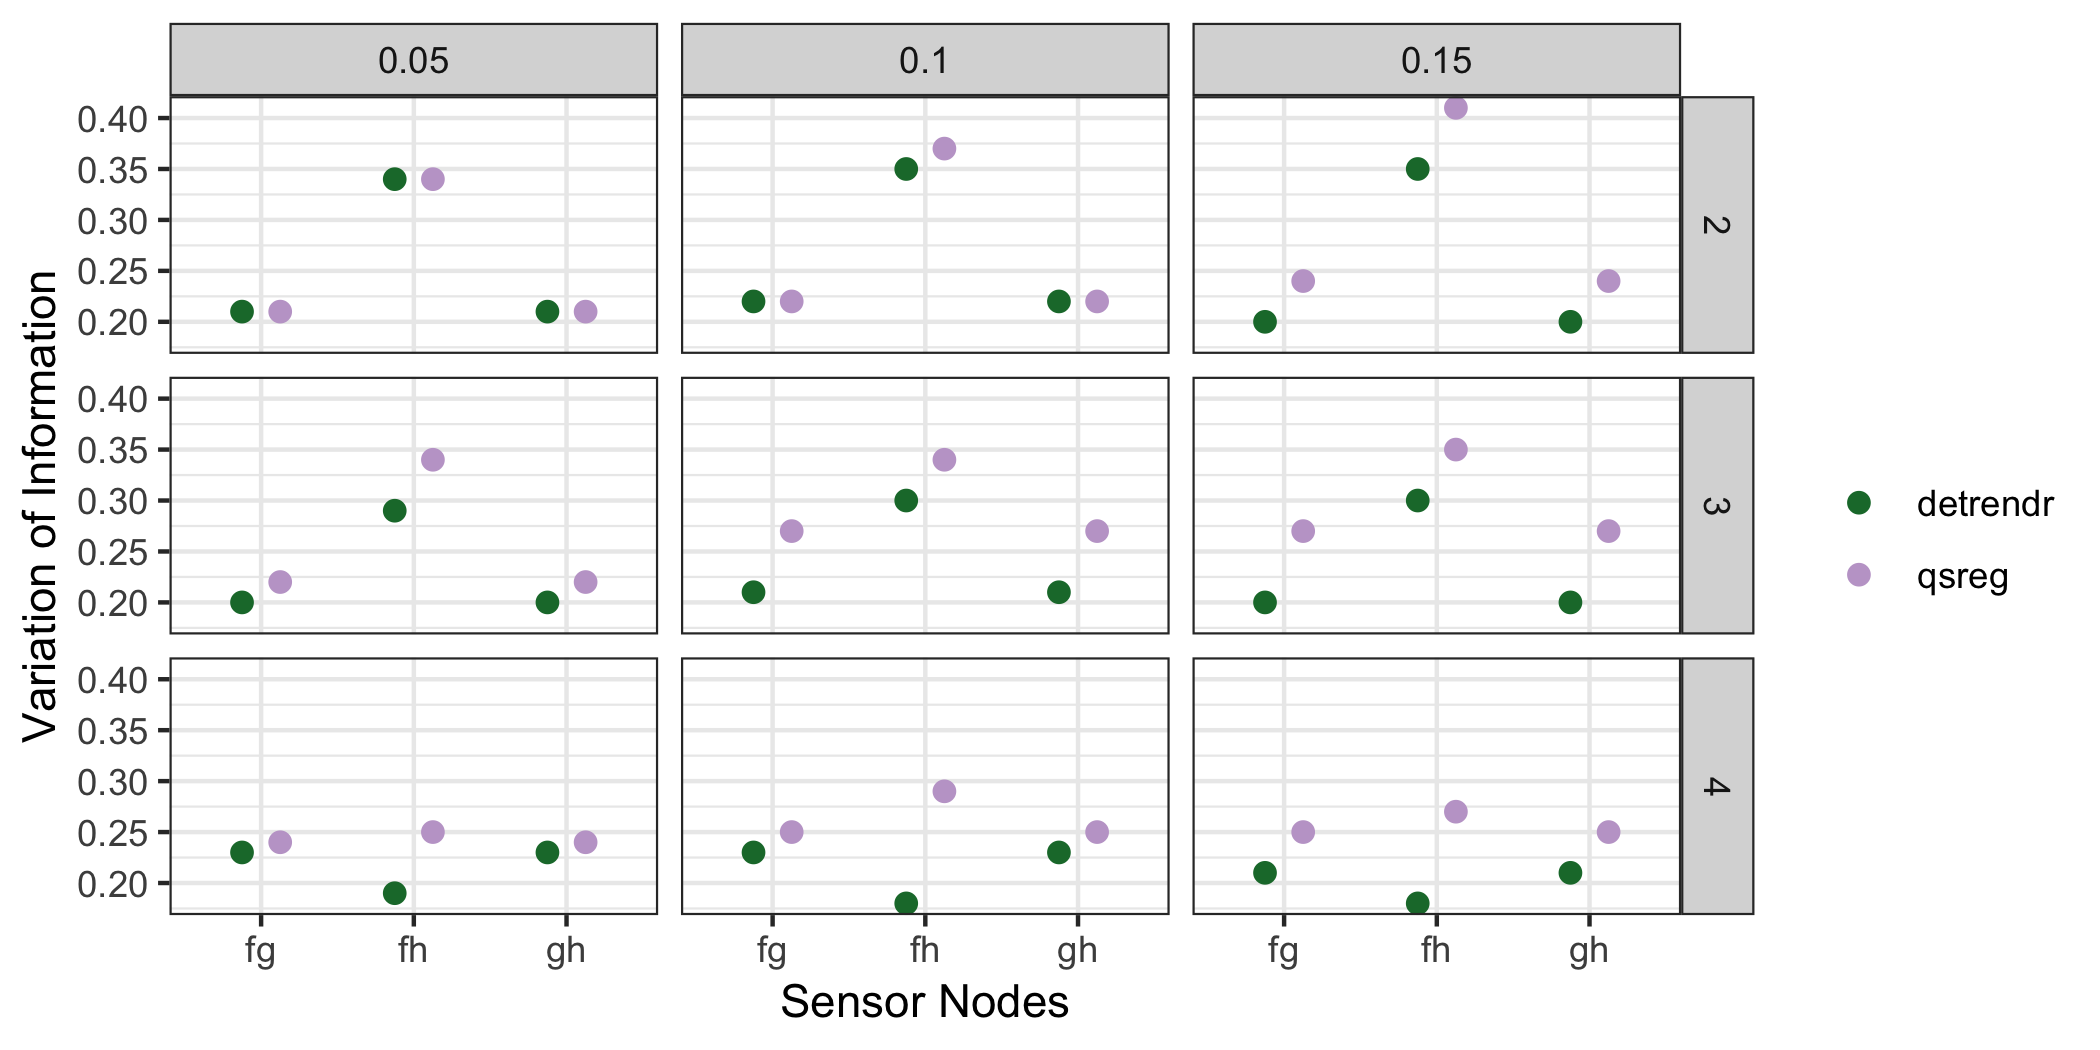
\includegraphics[width = .9\linewidth]{Figures/VI_app_short.png}
	\end{figure}
	
	
	\begin{figure}
		\caption{Rugplot showing locations of signal after baseline removal using detrendr estimate of 10th quantile.}
		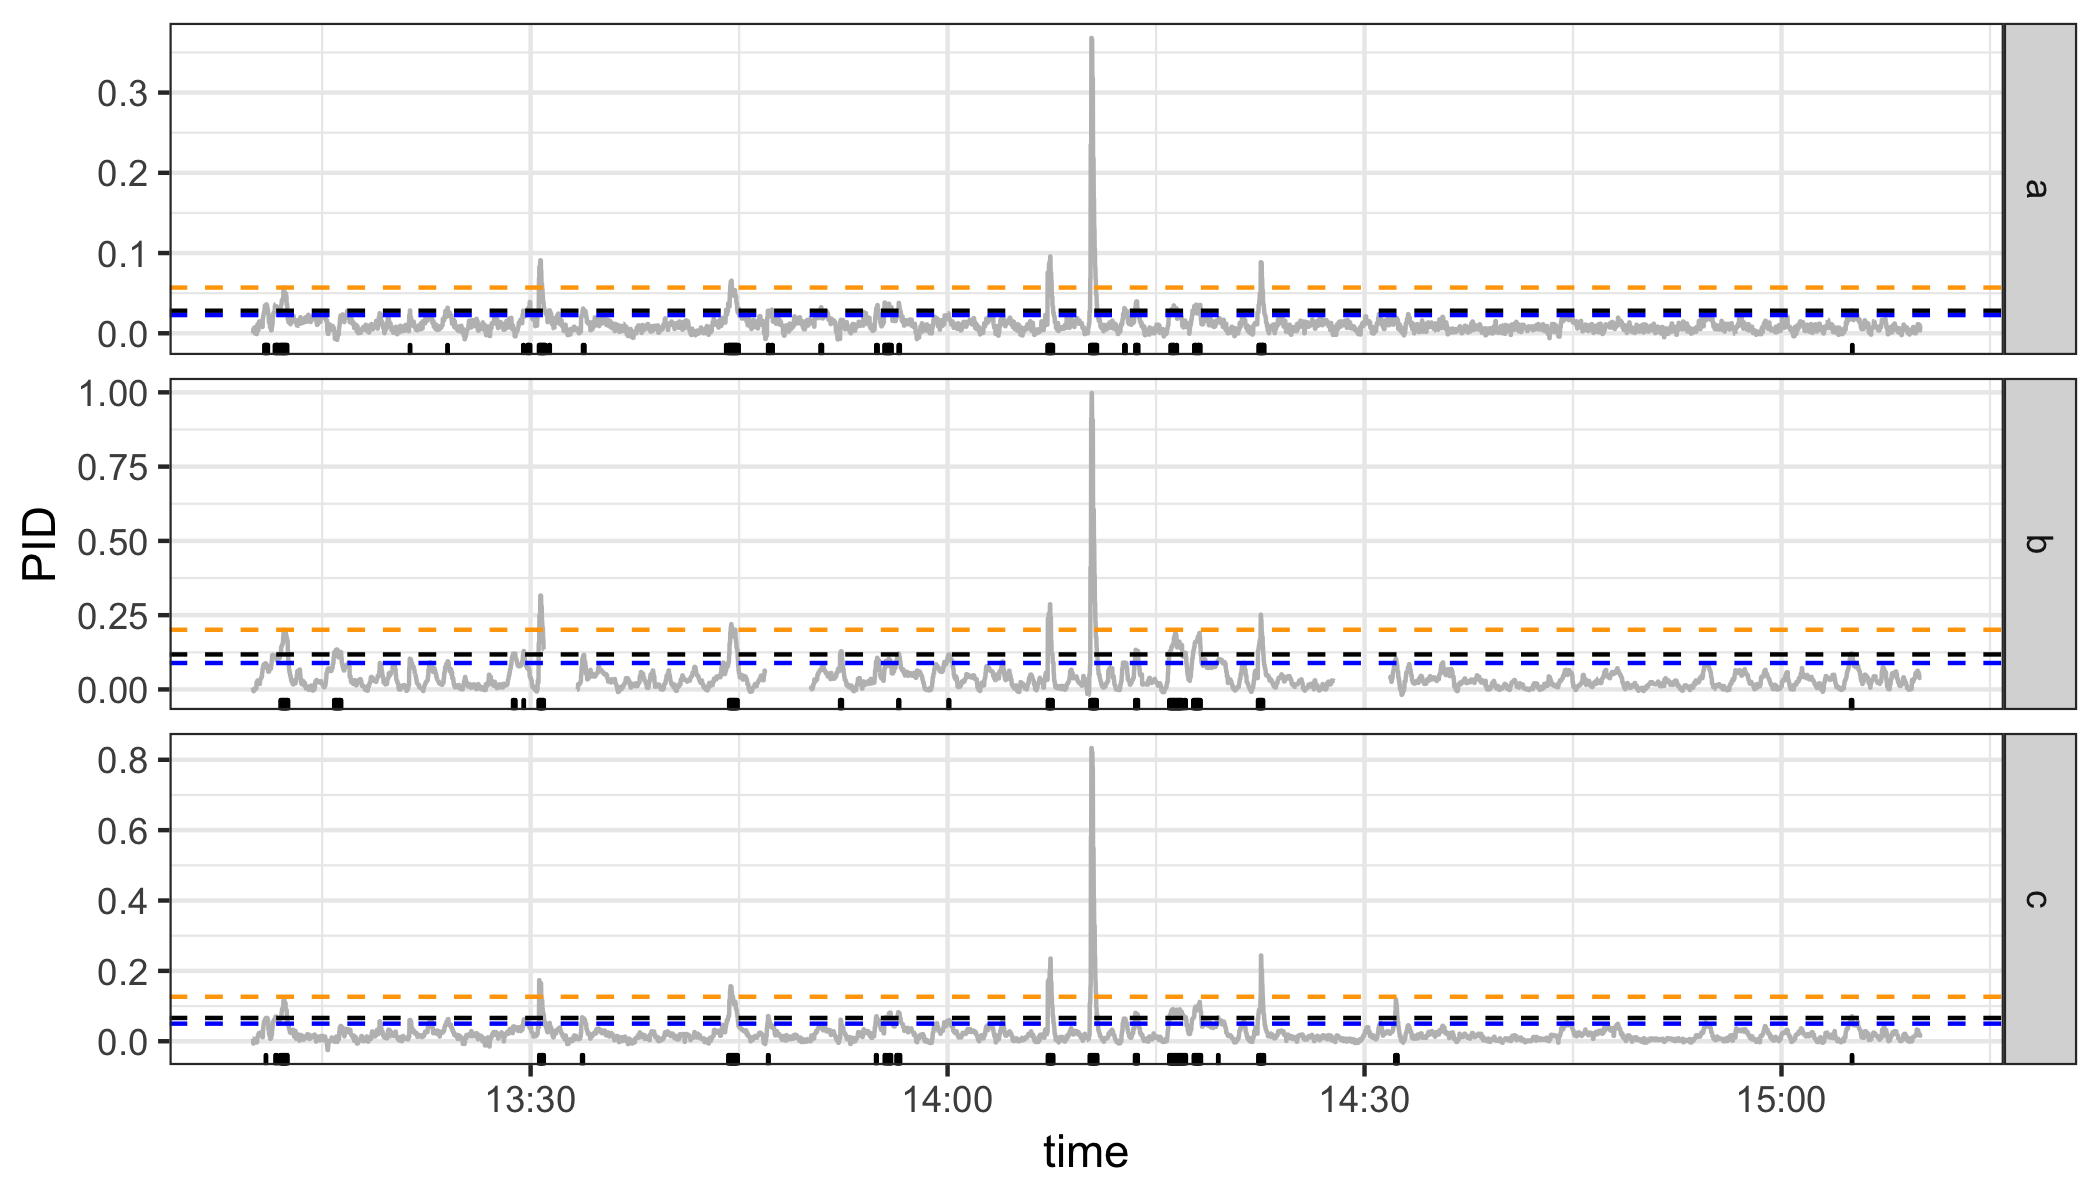
\includegraphics[width = \linewidth]{Figures/corrected_rugplot.png}
	\end{figure}

	
	Our windowed detrend method was used to removed the baseline drift from low cost air quality sensors so that the signal could be categorized using a simple threshold. The measurements were first standardized to have mean zero and variance 1. Three quantile levels for estimating the baseline trend were compared. The total dataset consisted of 52,322 observations per node. 
	The signal thresholds were set using the first 15,000 observations where it was known no signal was present. The thresholds were set as 3 times the standard deviation plus the mean of observations in this time period. The total number of seconds of signal for each node as well as the number of seconds where multiple nodes both reported signal is shown in Table 1. Table 2 shows the fraction of observations with different signal classifications by node combination. The BVI scores for the full dataset were 0.14, 0.13, and 0.14 for nodes f and g, f and h, and g and h, respectively. 
		
	\begin{figure}
		\caption{Low cost sensor data after drift removal using windowed detrend with eBIC.}
		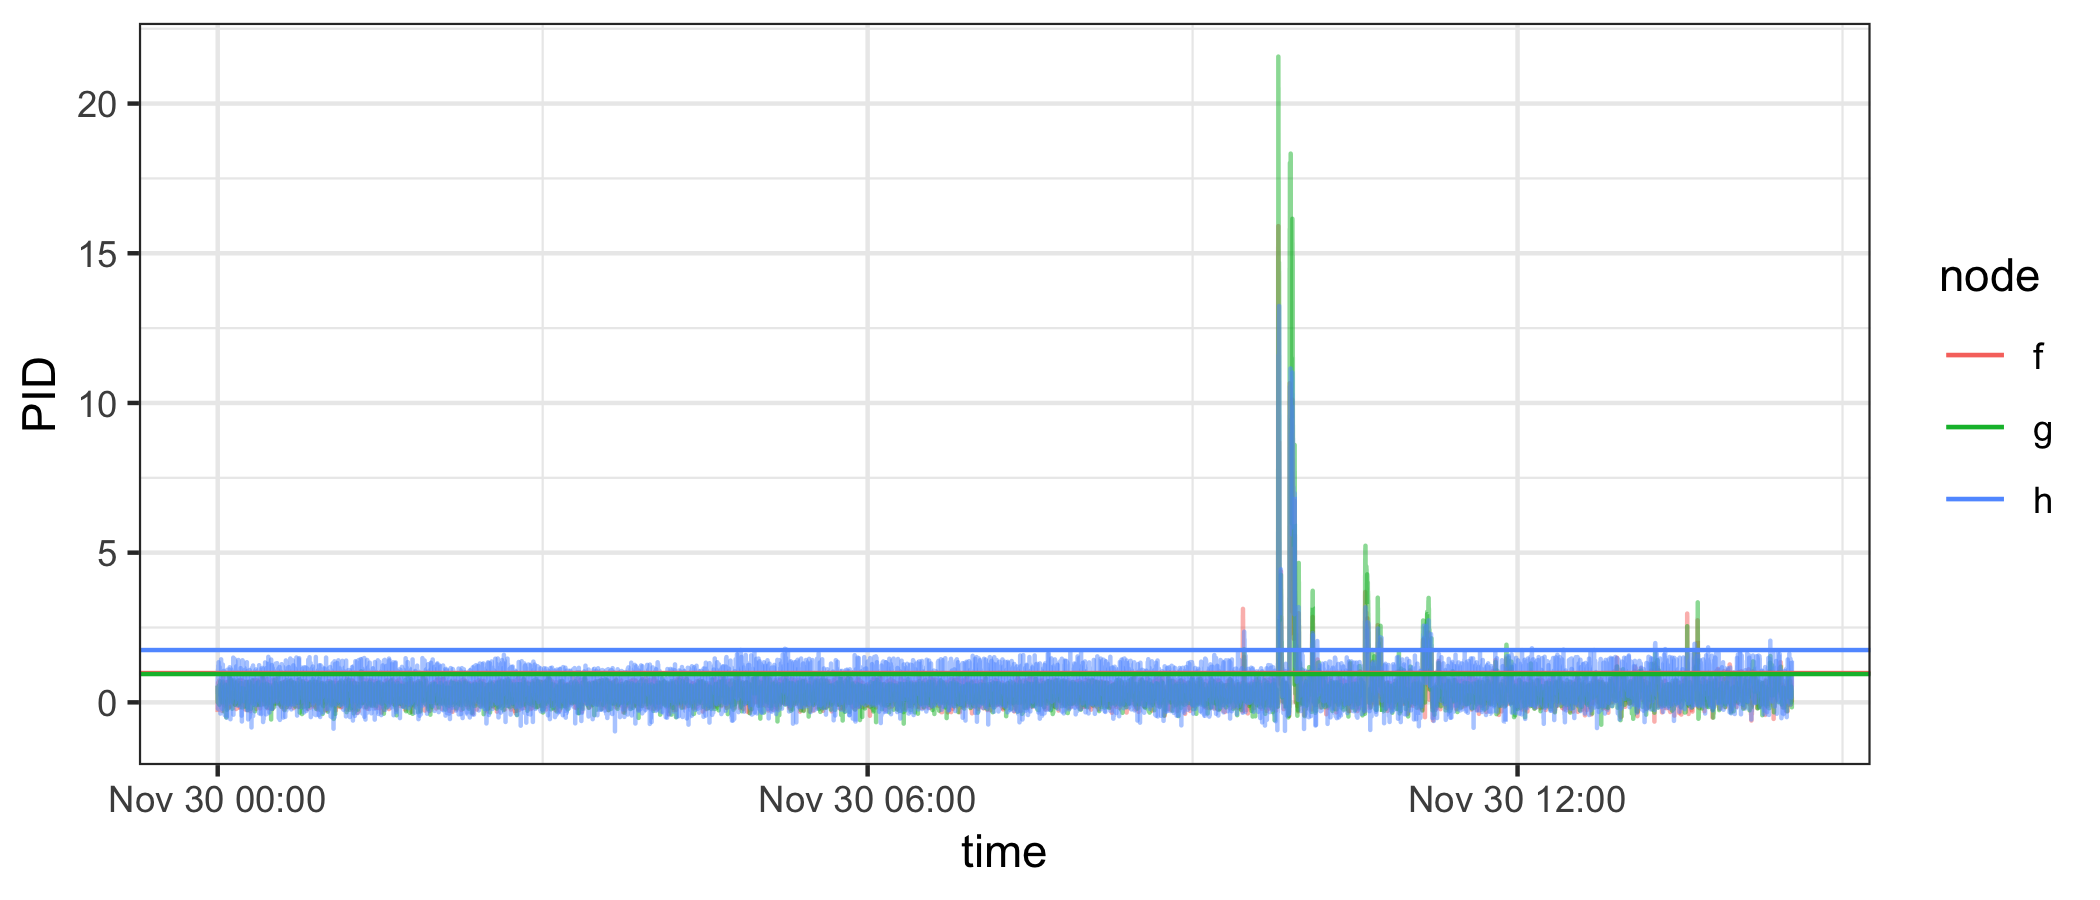
\includegraphics[width = \linewidth]{Figures/corrected_data.png}
	\end{figure}

	%latex.default(conf, file = "../Manuscript/full_confusion_detrend.tex",     rowlabel = "", rowname = c("f = 0", "f = 1", "f=0", "f=1"),     cgroup = c("h = 0", "h = 1"), rgroup = c("tau=0.05", "tau=0.1"),     n.rgroup = c(2, 2), colheads = rep(c("g = 0", "g = 1"), 2),     n.cgroup = c(2, 2), caption = "Confusion matrices for 3 SPod nodes after baseline removal (n=52322).")%
\begin{table}[!tbp]
\caption{Confusion matrices for 3 SPod nodes after baseline removal (n=52322).\label{conf}} 
\begin{center}
\begin{tabular}{lrrcrr}
\hline\hline
\multicolumn{1}{l}{\bfseries }&\multicolumn{2}{c}{\bfseries h = 0}&\multicolumn{1}{c}{\bfseries }&\multicolumn{2}{c}{\bfseries h = 1}\tabularnewline
\cline{2-3} \cline{5-6}
\multicolumn{1}{l}{}&\multicolumn{1}{c}{g = 0}&\multicolumn{1}{c}{g = 1}&\multicolumn{1}{c}{}&\multicolumn{1}{c}{g = 0}&\multicolumn{1}{c}{g = 1}\tabularnewline
\hline
{\bfseries tau=0.05}&&&&&\tabularnewline
~~f = 0&$51641$&$222$&&$1$&$  9$\tabularnewline
~~f = 1&$   23$&$190$&&$7$&$229$\tabularnewline
\hline
{\bfseries tau=0.1}&&&&&\tabularnewline
~~f=0&$51639$&$231$&&$1$&$  9$\tabularnewline
~~f=1&$   23$&$187$&&$7$&$225$\tabularnewline
\hline
\end{tabular}\end{center}
\end{table}
	
	

	\section{Conclusion}
	\label{sec:conc}
	
	
	\bigskip
	\begin{center}
		{\large\bf SUPPLEMENTARY MATERIAL}
	\end{center}
	
	\begin{description}
		
		\item[R-package for detrend routine:] R-package detrendr containing code to perform the diagnostic methods described in the article. The package also contains all datasets used as examples in the article. (GNU zipped tar file)
				
	\end{description}
	
	\section{References}

	
	\bibliographystyle{asa}
	\bibliography{detrendify}
	
\end{document}

